\chapter{Quantitative dark-field imaging}\label{ch:lung-dark-field}
Parts of this chapter are also presented in Abis M, Lovric G, Schittny J, Stampanoni
M, \emph{Quantitative lung microstructure mapping with X-ray dark-field grating interferometry on a laboratory source}.
\section{Introduction}\label{sec:introduction}
X-ray grating interferometry has been developed over the course of the last
fifteen years on both synchrotron and laboratory
sources~\parencite{David_2002,1347-4065-42-7B-L866,Weitkamp_2005,1347-4065-45-6R-5254,Pfeiffer2006}.
Interferometric imaging allows simultaneous access to three independent
images: the conventional absorption image, a differential phase signal and a
dark-field signal, also known as visibility contrast. This last signal has
been reported by multiple sources as being quantitatively linked to the
presence of unresolved structures in the sample, much smaller than the pixel
size of the detector, and typically of the order of the
micrometer~\parencite{Pfeiffer2008,Lynch:11,Yashiro:10}. Various clinically
relevant applications~\parencite{Wen_2009,Thilo2013} have been
proposed, including lung microstructural analyses~\parencite{Schleede17880,Meinel_2014,Meinel_2013,Yaroshenko_2013}.

In particular, emphysema is a pathological condition of the lung
resulting in structural changes in the alveoli, that is at the smallest
hierarchical level in the tissue. These changes are caused by the
destruction of interalveolar septa, with larger air spaces progressively
replacing the fine architecture of the lung
parenchyma~\parencite{Sharafkhaneh_2008}. These larger spaces have a less
favorable surface-to-volume ratio, thus lowering the efficiency
of respiratory exchanges. Absorption radiography proved to be accurate in
diagnosing emphysema only in the advanced stages of the disease. 
High-resolution computed tomography is able to detect regions in the lung
with abnormally low attenuation, at the cost of exposing the patient
to a higher radiation dose.

Previous studies on murine lungs established that the increased sensitivity of
the dark-field signal of an X-ray grating interferometer to micrometer-sized
features can distinguish between emphysematous from healthy samples and
provide a mapping of the parenchyma showing the localization of the
structural damage.
The strength of the dark-field signal in grating interferometry is
given by the small-angle scattering of X-rays by structures smaller than the
spatial resolution of the imaging system. The lung is therefore an ideal
application for this technique, since the alveoli are much
smaller than the spatial resolution available for chest radiography.

An application of this alternative contrast mechanism to detect 
structural changes in the lungs to the early detection of lung cancer is
also possible. Lung cancer is commonly diagnosed through chest radiography,
which has a low sensitivity in the early stages of the disease, below \SI{50}{\percent} for a mean tumor size of
\SI{19}{\milli\meter}~\parencite{Fardanesh2012,doi:10.1148/radiol.11100153}.
Our technique demonstrates a quantitative connection between the measured
dark-field signal and specific structure sizes in the lung parenchyma, and
could therefore be applied to screening and early-stage detection of nodules in
the lung with an abnormal composition.

In this work we present a quantitative model of the dark-field signal
generated by lung tissue in an X-ray grating interferometer on a laboratory
source. High-resolution tomographic data resolving the features down to single
alveoli is analyzed with established post-processing techniques to extract a
ground truth on the sizes of the structures composing the lung tissue. The
lung is then modeled as a suspension of spheres of different sizes in a
homogeneous medium, in the hypothesis that the signals generated by spheres
of different sizes and by X-rays of different energies sum up incoherently.
Finally, an X-ray interferometric radiography on a laboratory source is
recorded, to allow a direct comparison between the expected dark-field
signal calculated according to this model and the experimental values.

\section{A two-dimensional laboratory setup}
A new set of gold gratings for a face-on grating interferometer was designed
in collaboration with the Karlsruhe Institute of Technology, specializing in
the production of this kind of microstructures. The design parameters were
relaxed when compared to the previous chapter~\ref{ch:edgeon}. The main goal
of this chapter is pushing the limits of face-on Talbot-Lau
interferometry on a laboratory source, while still keeping the speed of
two-dimensional image recording, avoiding the scanning procedure of a
collimated beam described in section~\ref{sec:edge-on-arrangement}.

The same constraints on the aspect ratio of the absorption gratings are
still relevant, however, and a minimum thickness of \SI{100}{\micro\meter}
is required, as this equals one attenuation length for gold at \SI{100}{\kilo\eV}.
This is a thickness sufficient to reduce the intensity of the incoming beam
by a factor of $\exp(-1)$. Fabrication
techniques~\parencite{David2007,Kenntner2010} can achieve aspect ratios below
\num{60}, it was chosen to specify a period of \SI{5.4}{\micro\meter}. This
translates to an aspect ratio of \num{40}.

Given the relatively strong transmission through the grating lines at higher
energies, the source voltage is limited to~\SI{100}{\kilo\voltpeak}. The
spectrum, simulated with the SpekCalc software~\parencite{spekcalc} is shown in
figure~\ref{fig:spectrum-100kV}.

\begin{figure}[htb]
    \centering
    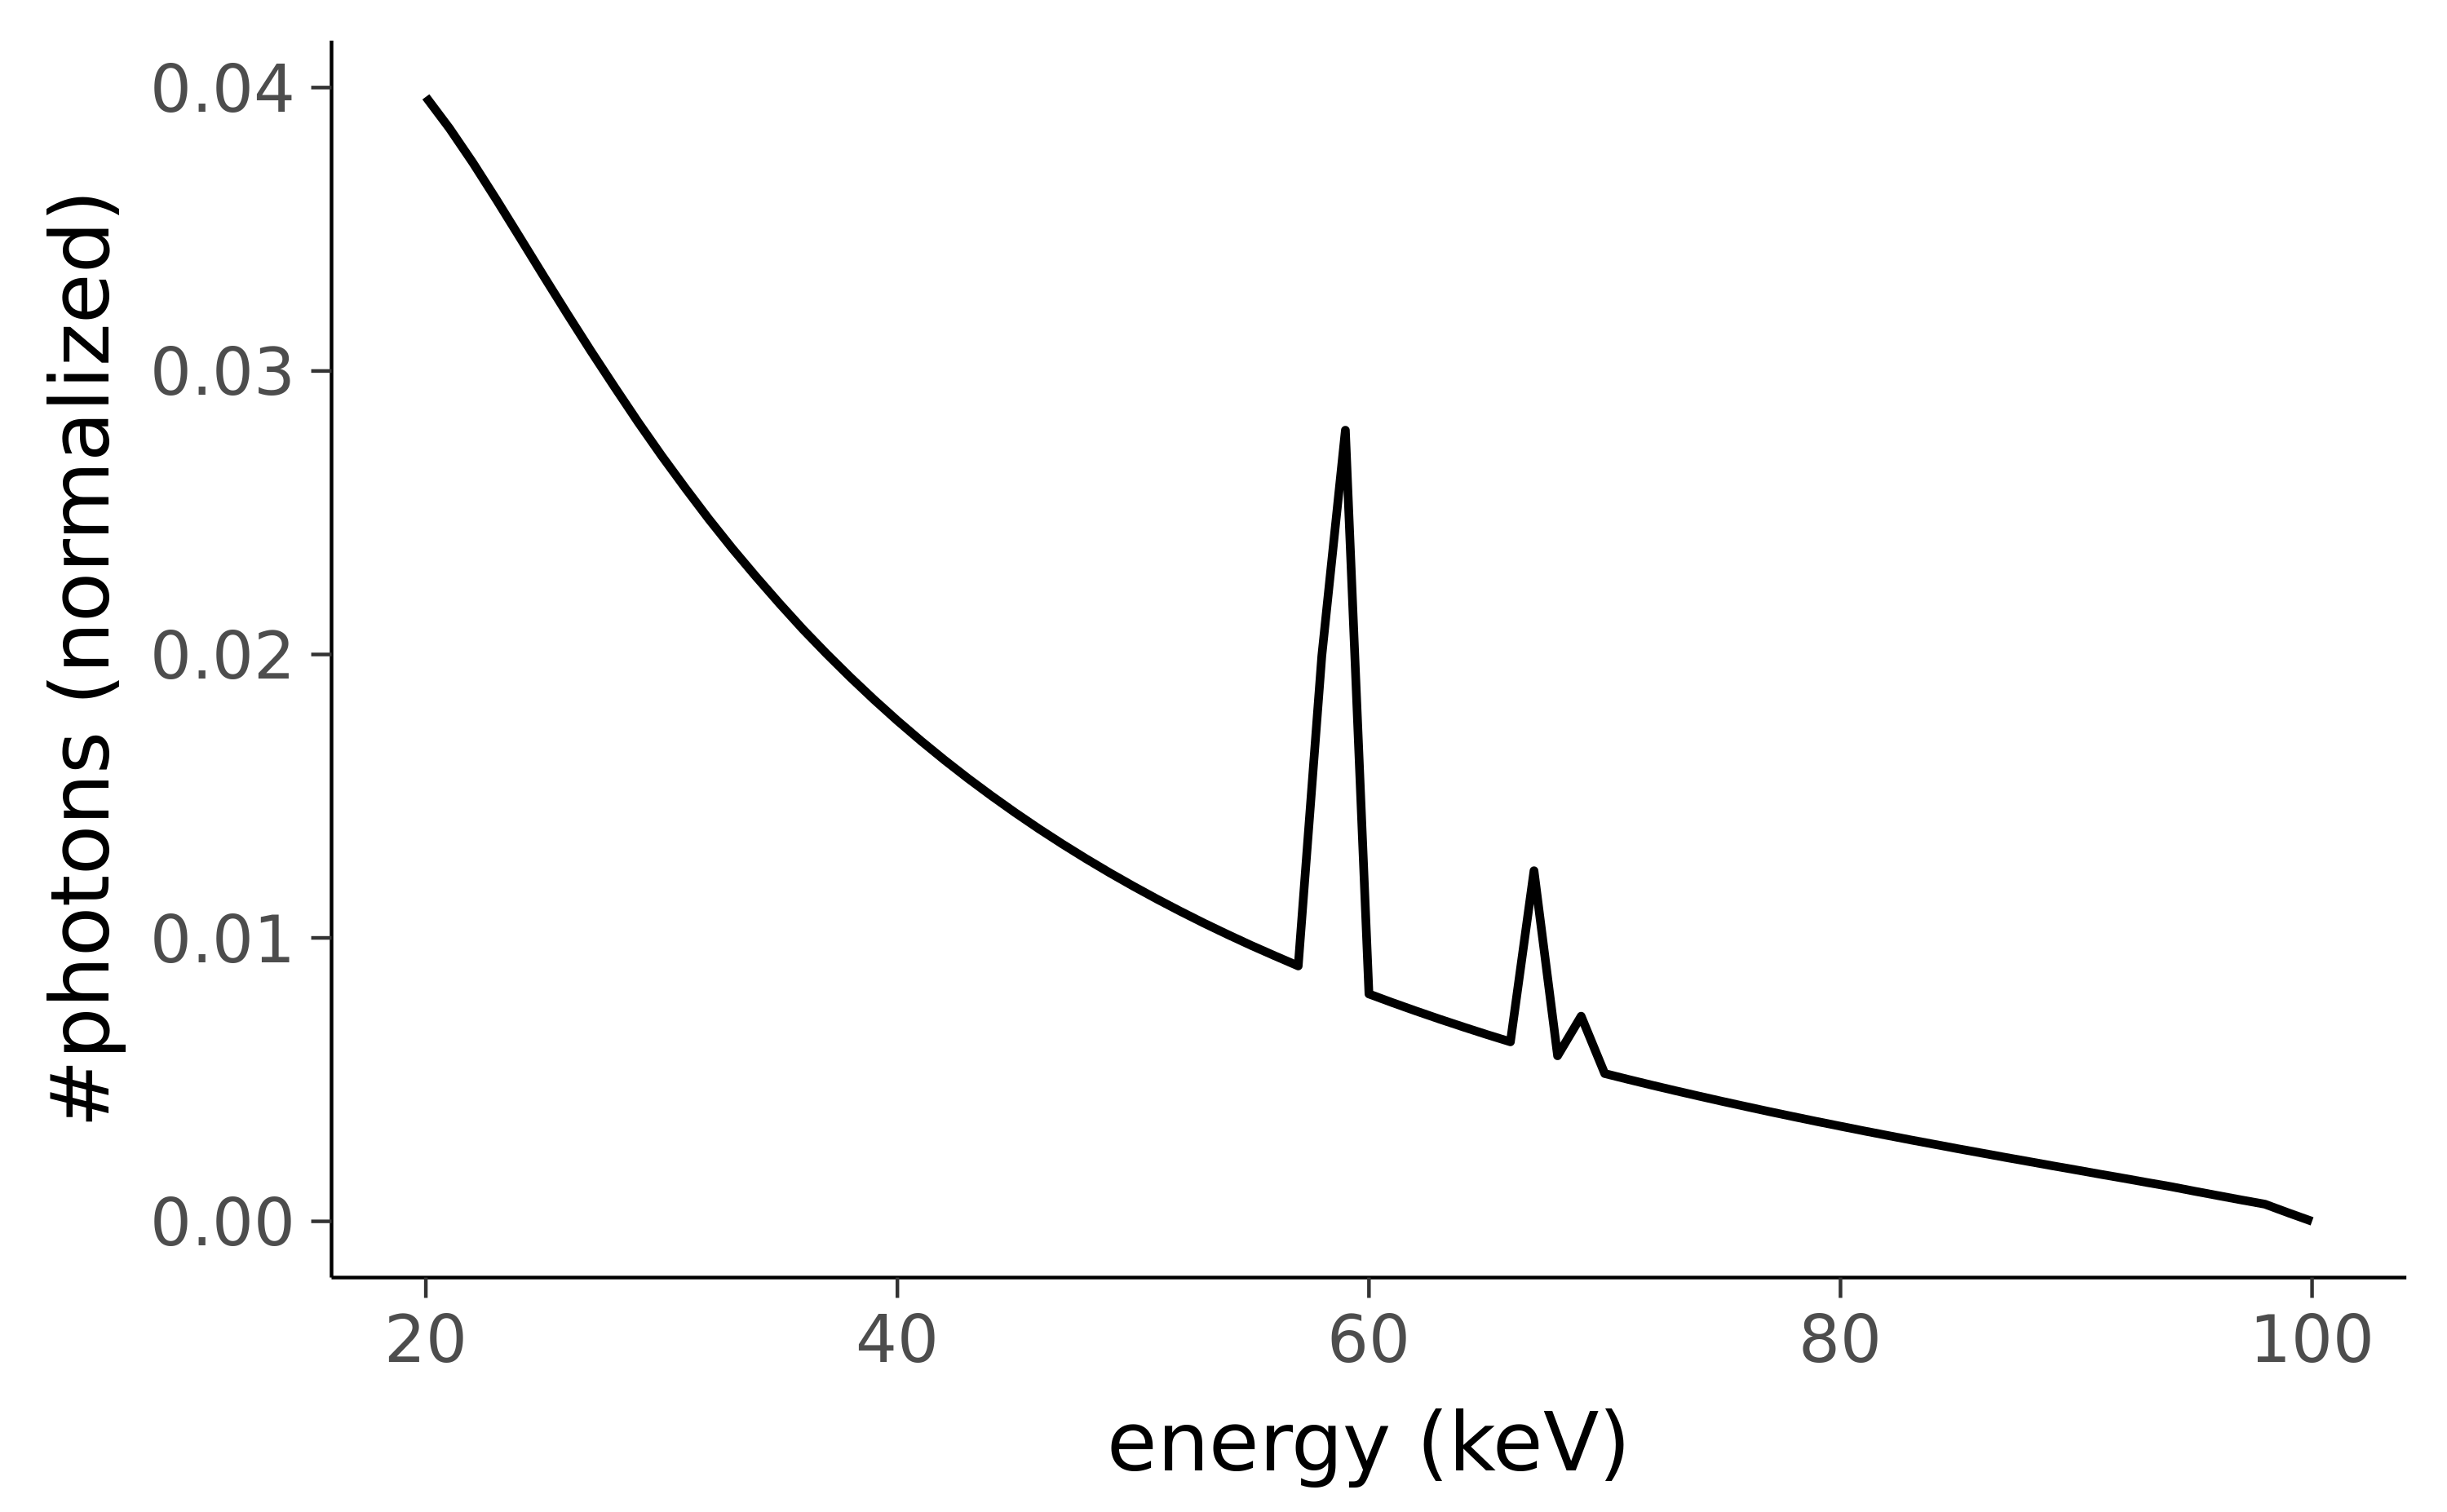
\includegraphics[width=\textwidth]{gfx/spectrum-visibility/spectrum-100kV.png}
    \caption[Spectrum of the laboratory source at \SI{100}{\kilo\voltpeak}]{Spectrum of the laboratory source with an acceleration voltage of
        \SI{100}{\kilo\volt}. Simulated with the SpekCalc
        software~\parencite{spekcalc}.}
    \label{fig:spectrum-100kV}
\end{figure}

In turn, this limitation implies a lower average energy of the beam.
Therefore a design energy of~\SI{45}{\kilo\eV} was chosen for the
$\pi$-shifting \G1. The setup is again symmetric, operating at the first
Lohmann order to benefit from the widest spectral acceptance. The
intergrating distance is calculated with
equation~\eqref{eq:lohmann-distance} and magnified as in
equation~\eqref{eq:magnification-distance}

\begin{equation}
    D_1^\prime = 2\frac{p^2}{8\lambda} =
    \frac{(5.4)^2\si{\micro\meter\squared} \cdot \SI{45}{\kilo\eV}}{4
        \cdot 1.24 \cdot 10^{-3}\si{\micro\meter\kilo\eV}} =
        \SI{26}{\centi\meter}.
    \label{eq:intergrating-distance}
\end{equation}

\section{Silicon and cadmium telluride detectors}

The first detector available to us for two-dimensional radiography experiments is
an Eiger 1M module by Dectris Ltd~\parencite{dectris-eiger, 1748-0221-9-05-C05032}. It features a silicon sensor
with a thickness of~\SI{450}{\micro\meter} and a pixel size of
$75\times\SI{75}{\micro\meter\squared}$. The efficiency of this sensor is
shown in figure~\ref{fig:eiger-efficiency}, and it is clear that it is not
very suitable for this kind of high-energy experiments since it does not
provide enough quantum efficiency --- less than \SI{10}{\percent} above
\SI{30}{\kilo\eV}.

\begin{figure}[htb]
    \centering
    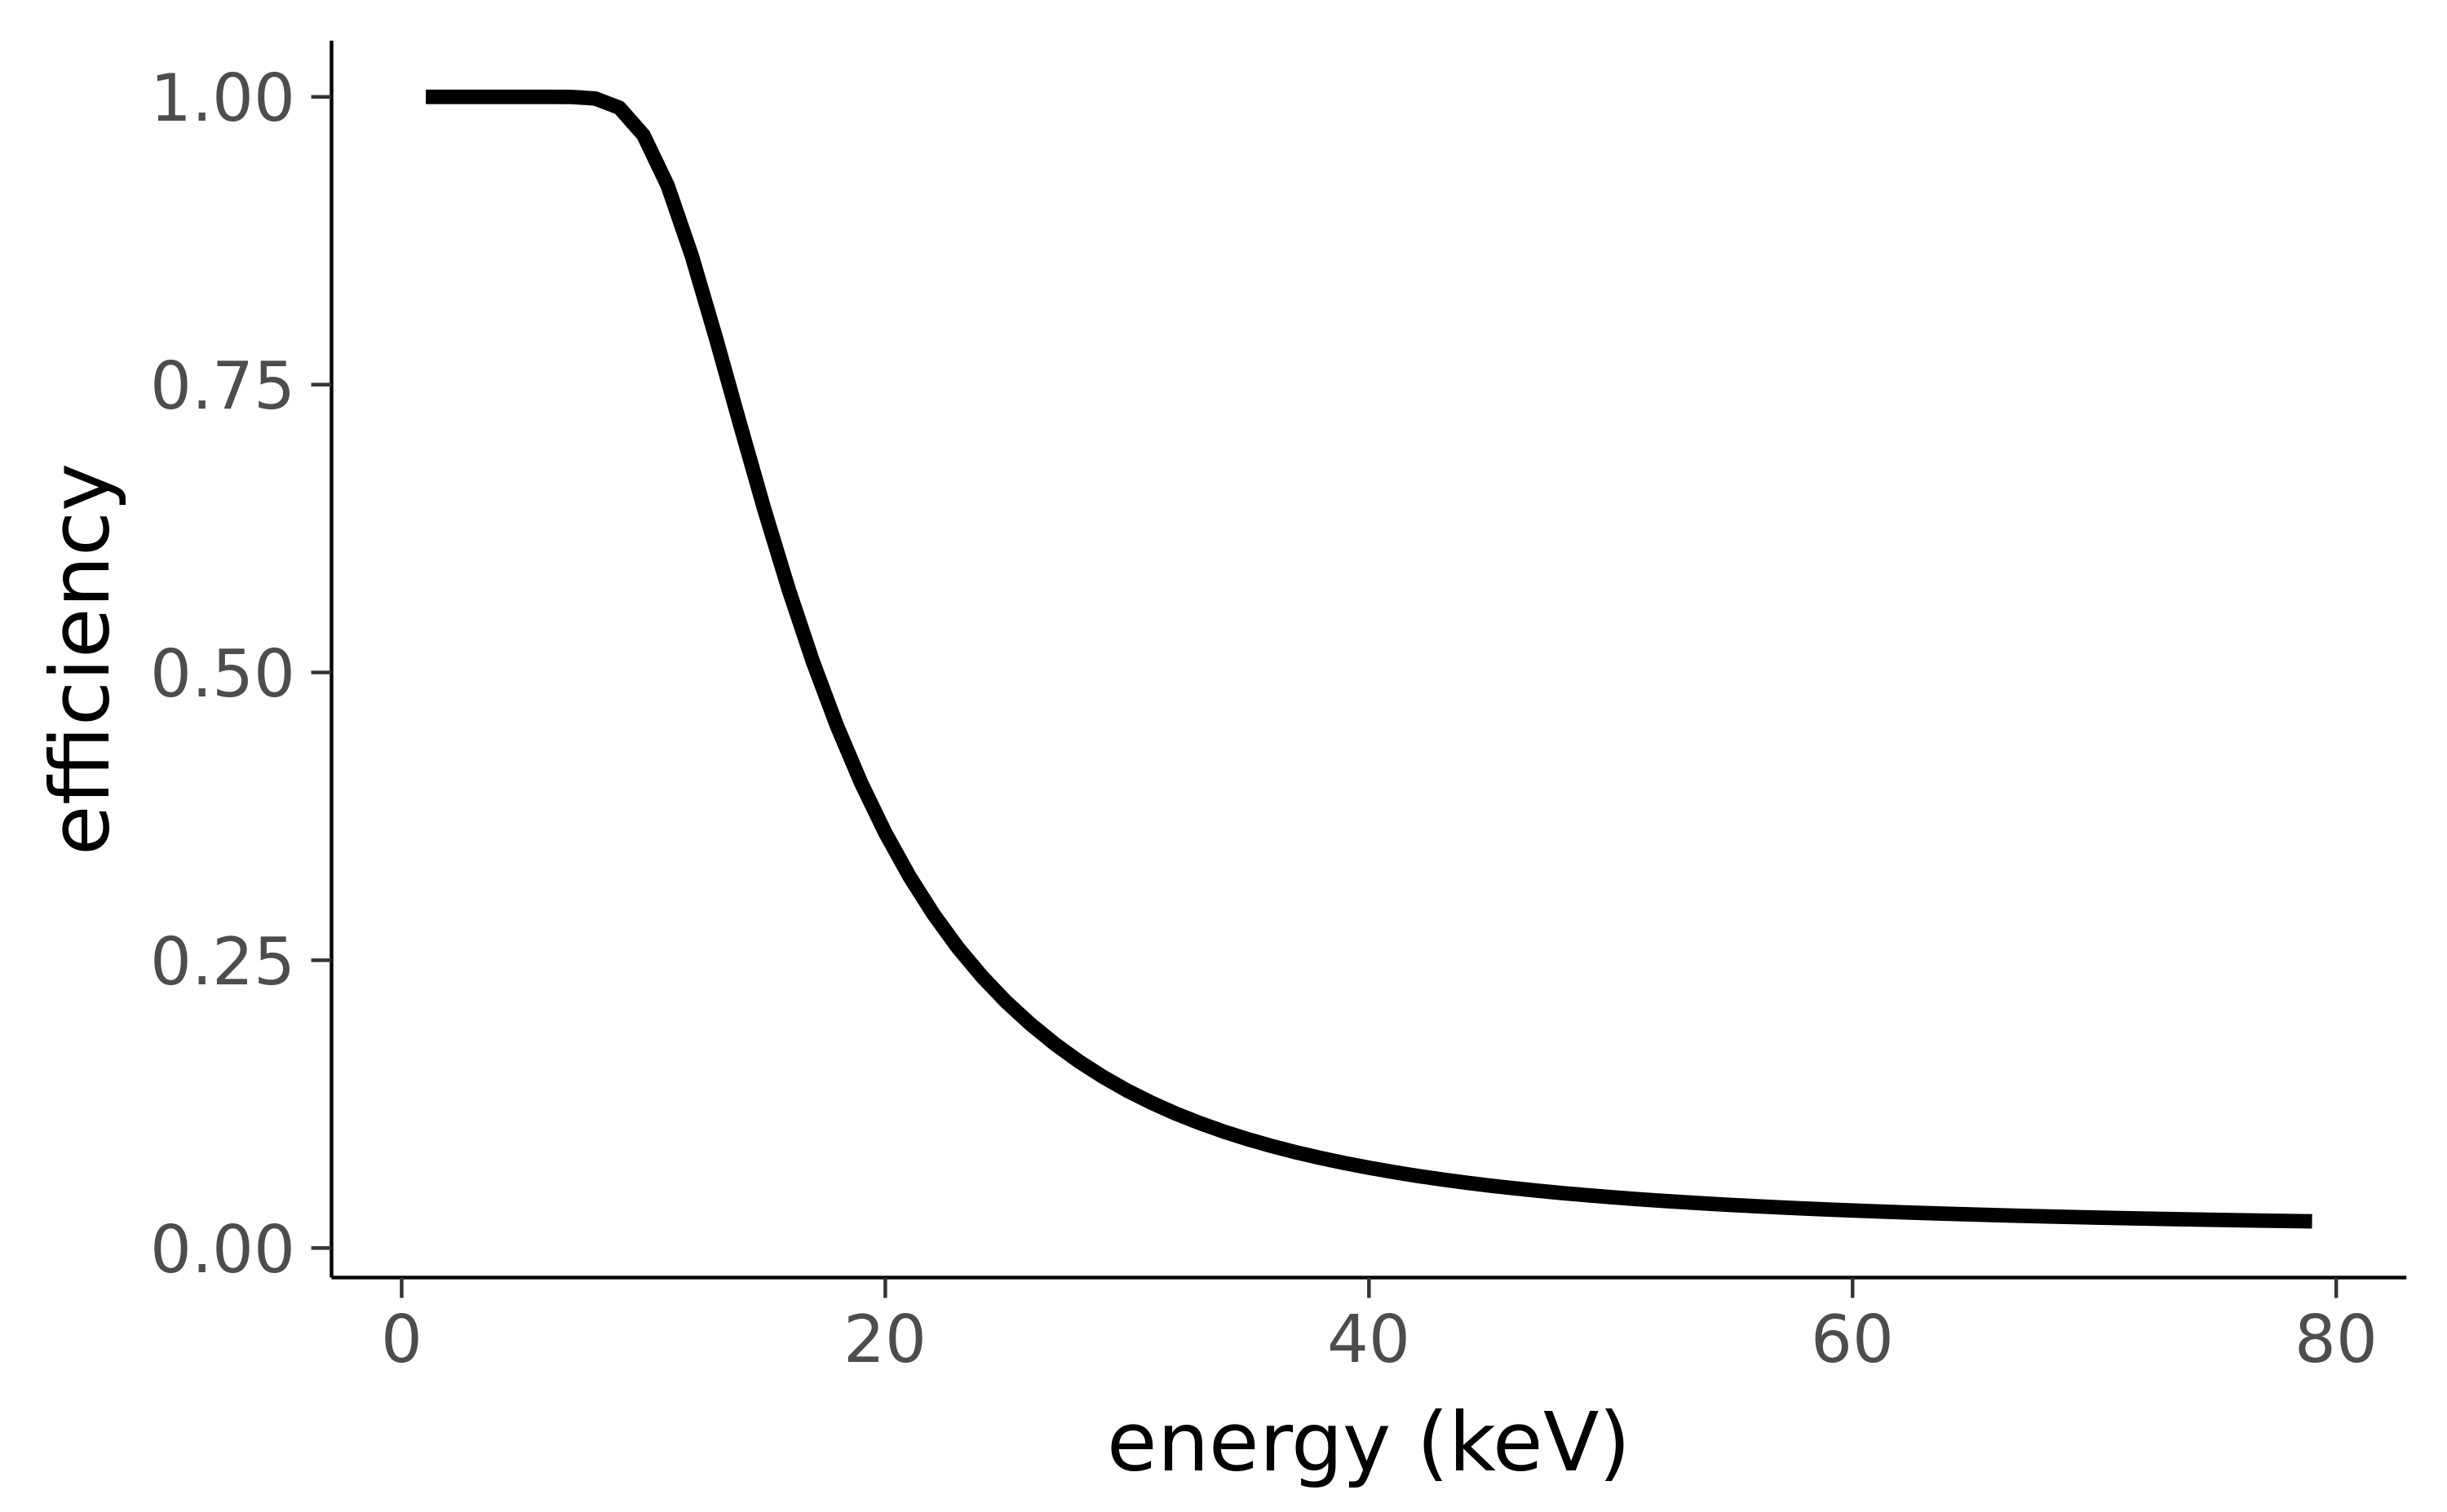
\includegraphics[width=\textwidth]{gfx/eiger/efficiency.png}
    \caption[Efficiency of the Eiger silicon detector]{Efficiency of the \SI{450}{\micro\meter} thick sensor of the
Eiger 1M detector as a function of energy.}
    \label{fig:eiger-efficiency}
\end{figure}

Nevertheless, it could be used for imaging a chicken paw, shown in
figure~\ref{fig:eiger-chicken}.

\begin{figure}[htb]
    \centering
    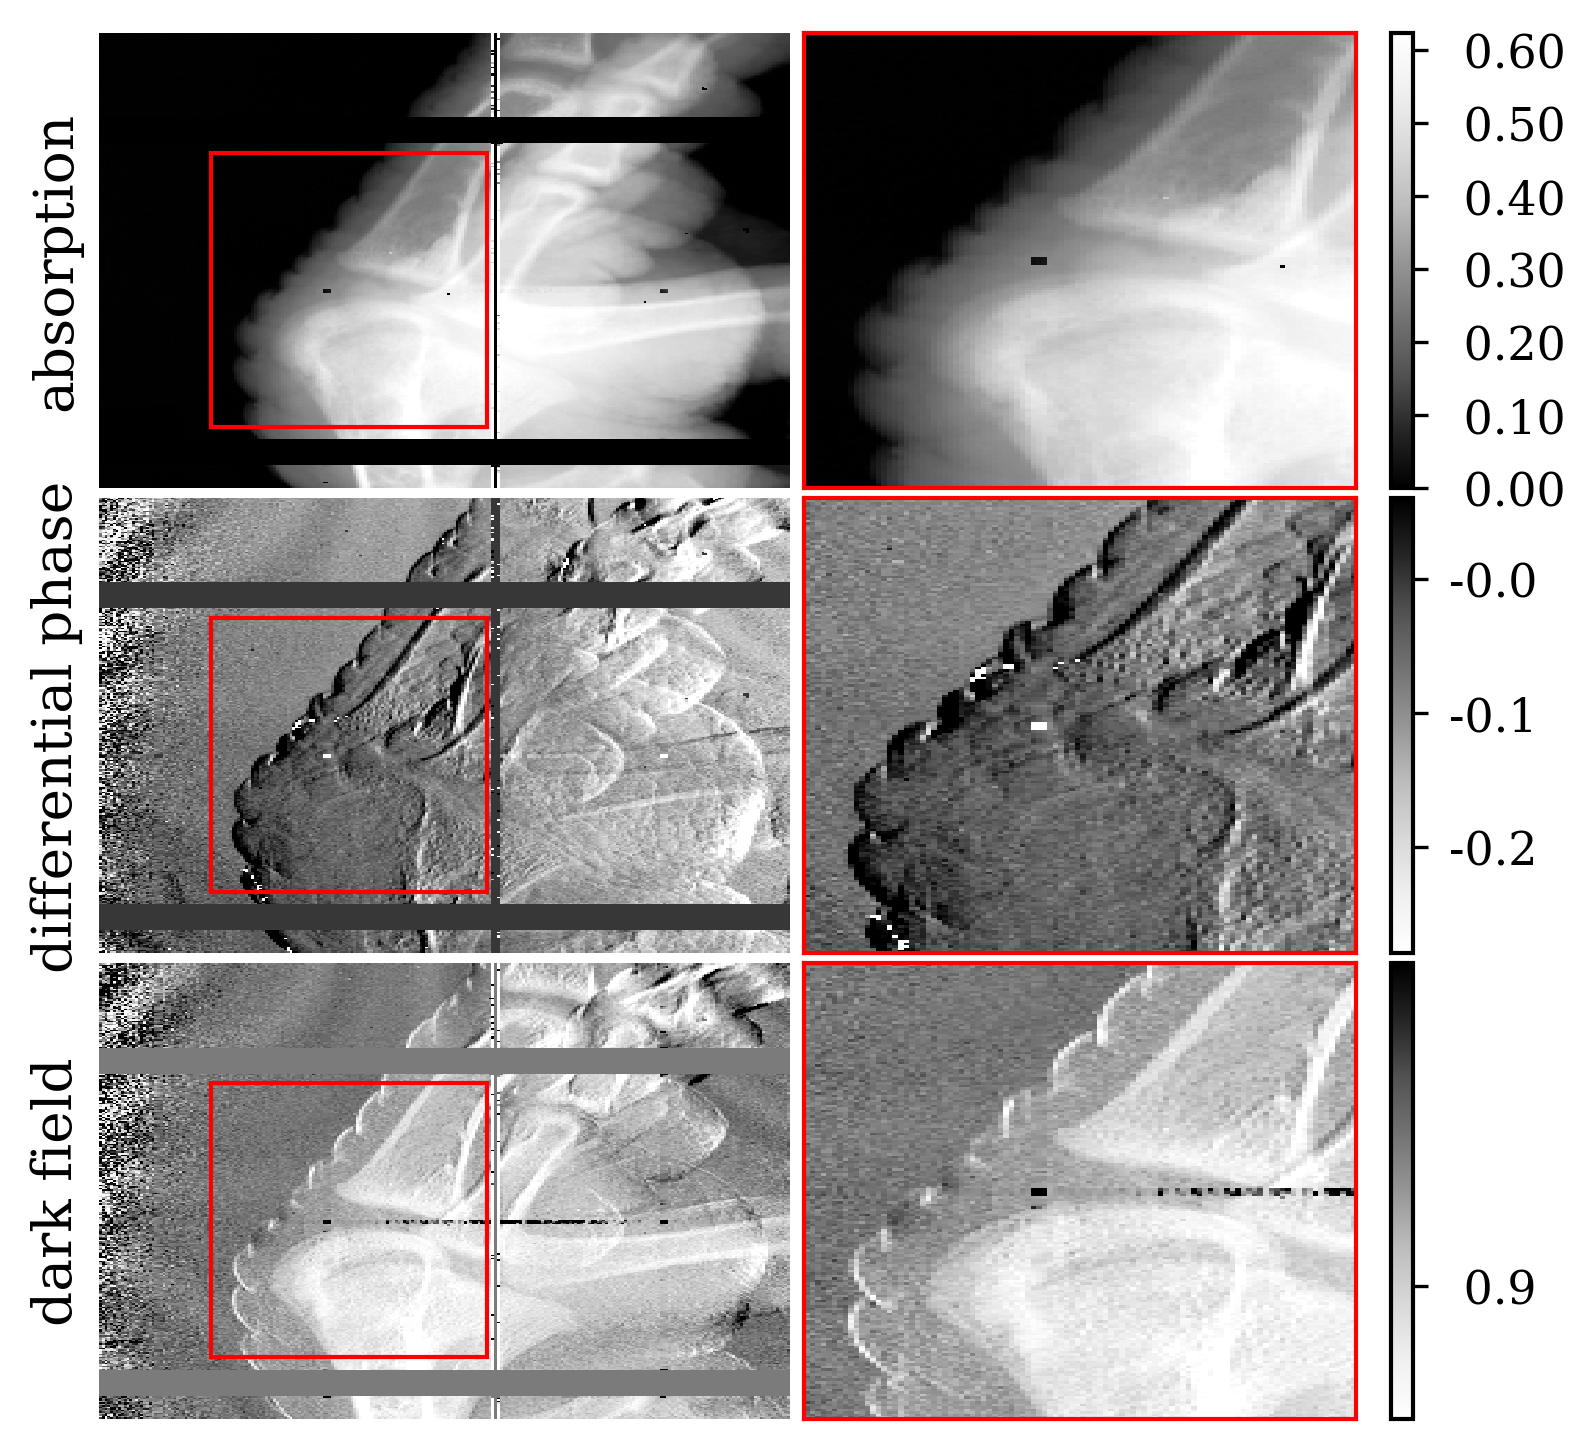
\includegraphics[width=\textwidth]{gfx/eiger/series_160729_170729669658_series_160729_171501073073.png}
    \caption[Chicken paw radiography]{Chicken paw scanned with a \SI{45}{\kilo\eV} two-dimensional
grating interferometer and the silicon detector Eiger 1M.}
    \label{fig:eiger-chicken}
\end{figure}

Unfortunately, imaging with this detector is unadvisable, as not only the lack of efficiency to
high-energy photons negatively impacts the visibility and the exposure
times, but the photons that go through the sensor are able to cause
radiation damage in the electronic boards of the detector itself.

For these reasons, another detector, a prototype based on Santis CdTe by
Dectris Ltd., was used. The cadmium
telluride sensor with a thickness of \SI{750}{\micro\meter} provides high
quantum efficiency at high energies (>\SI{90}{\percent} at
\SI{60}{\kilo\eV}) with a pixel size of
$75\times\SI{75}{\micro\meter\squared}$. 

The average visibility of the interference pattern without any
sample is 14\% (figure~\ref{fig:visibility-titlis}). The source is a Comet
MXR-225/26 X-ray tube operated at \SI{100}{\kilo\voltpeak} and
\SI{6}{\milli\ampere}. The source size is \SI{1}{\milli\meter}.
The phase-stepping procedure was performed with 31 phase steps with 1 s
exposure per step.

\begin{figure}[htb]
    \centering
    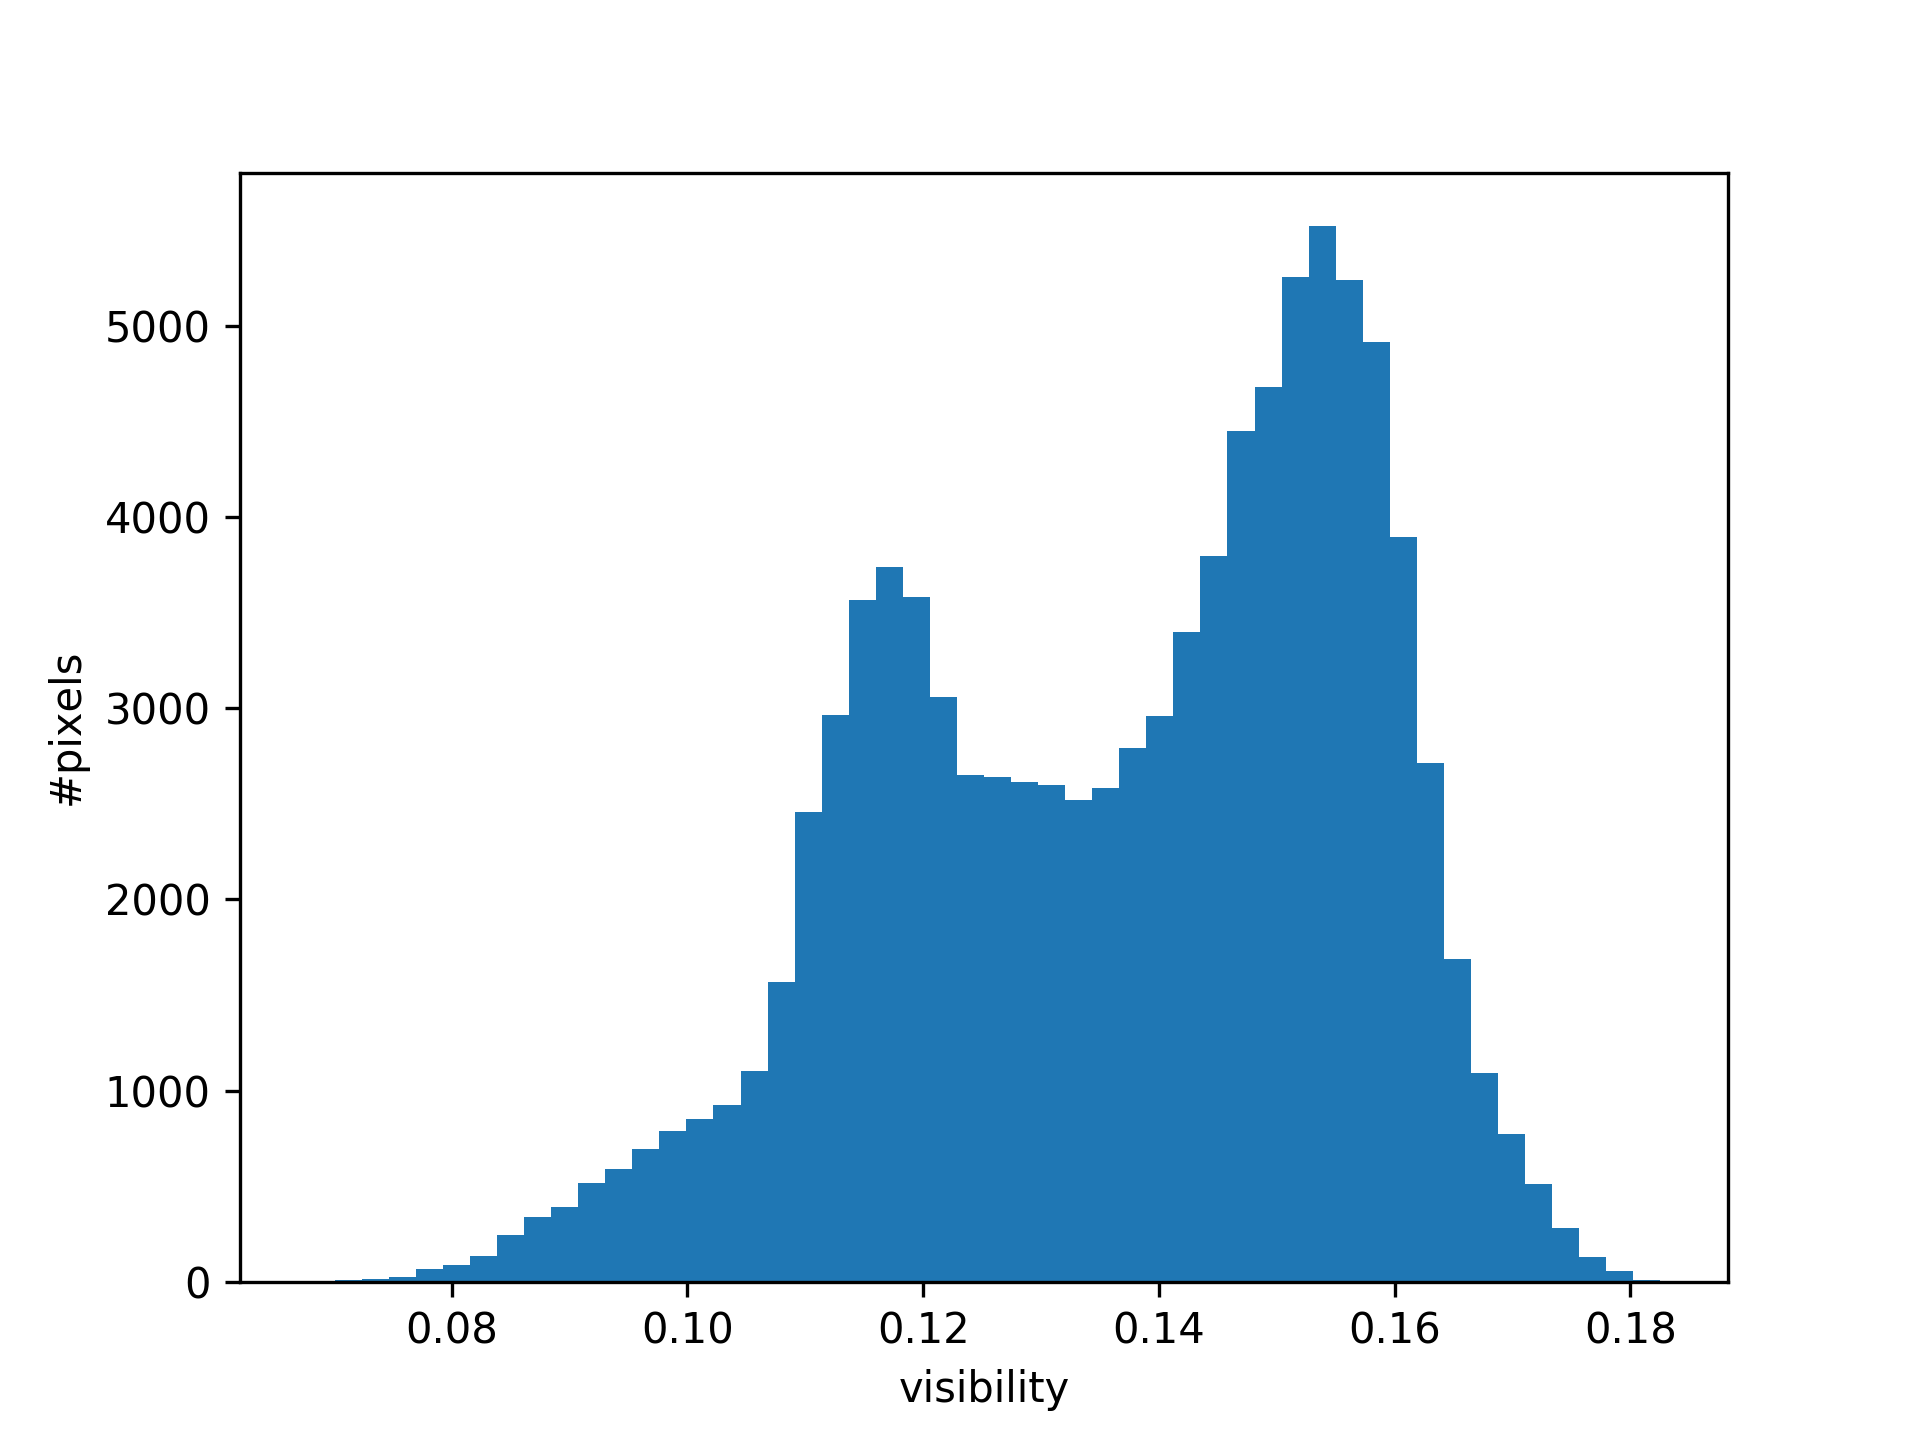
\includegraphics[width=.8\textwidth]{gfx/visibility_titlis.png}
    \caption[Visibility of the face-on interferometer]{Visibility histogram of the face-on interferometer with a
        design energy of~\SI{45}{\kilo\eV} on a cadmium telluride prototype
        sensor. The average is
        \SI{14}{\percent}.}
    \label{fig:visibility-titlis}
\end{figure}

The setup is shown in figure~\ref{248327}.

\begin{figure}[htb]
    \centering
    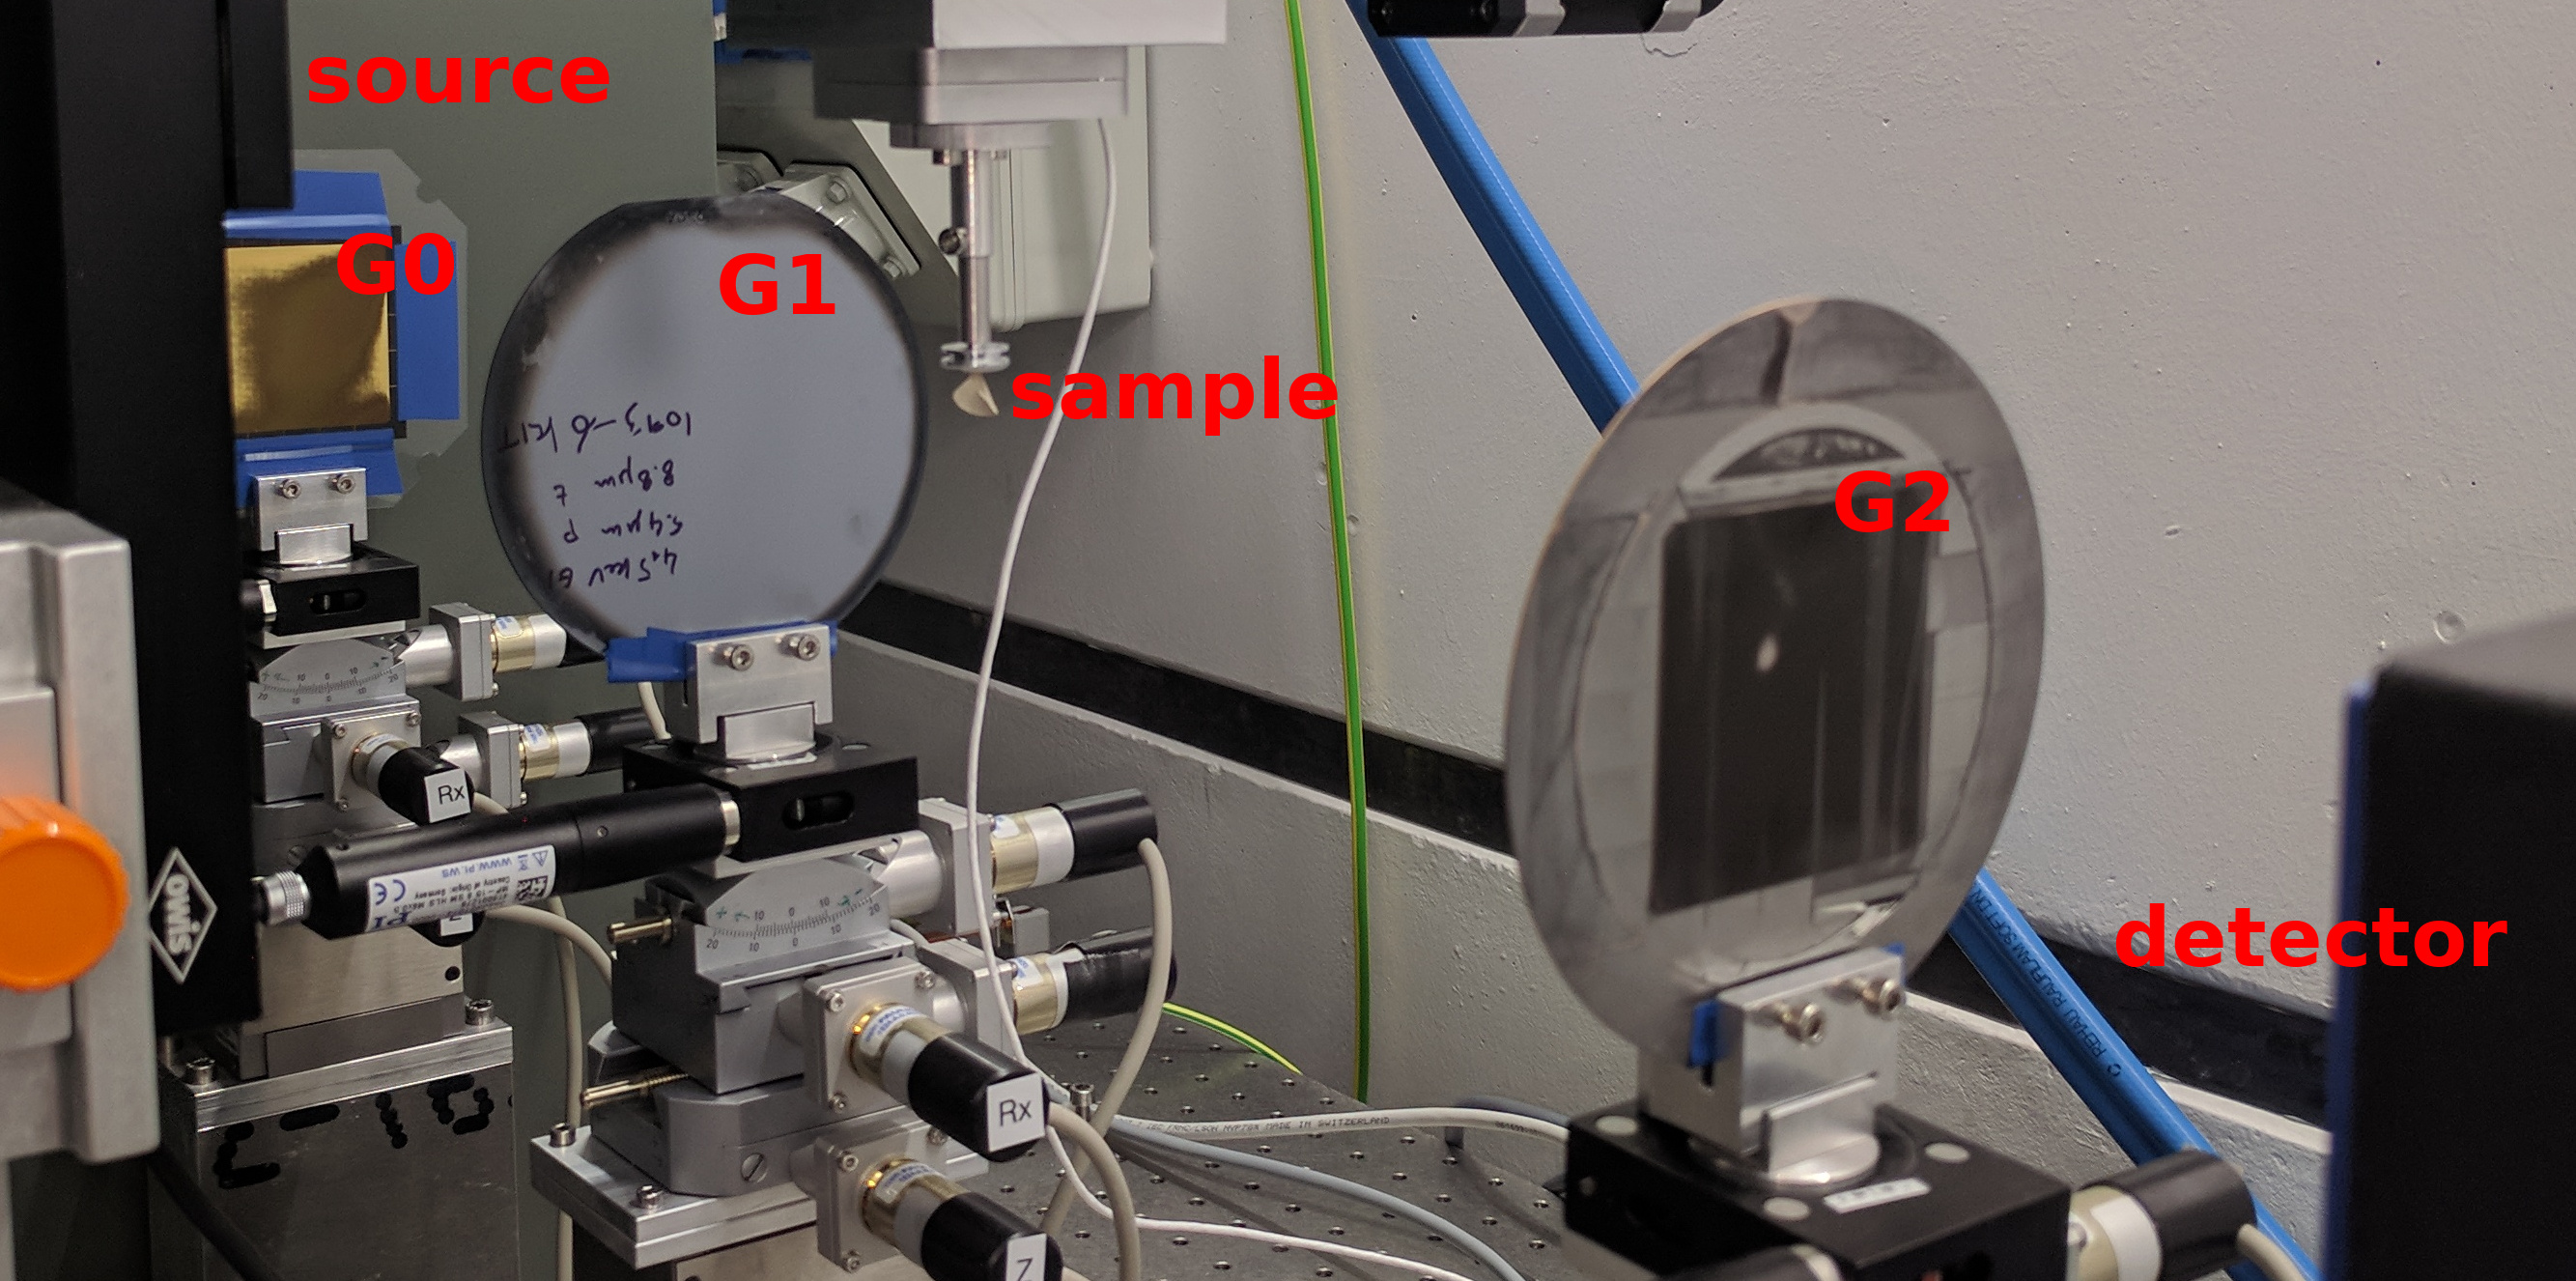
\includegraphics[width=0.70\columnwidth]{gfx/lung-paper-figures/lung-setup/lung-setup}
    \caption[Photo of the Talbot-Lau interferometer for lung radiographies]{Talbot-Lau interferometer with three gratings G0, G1 and G2, used for
        the radiographies on the laboratory source.
        {\label{248327}}%
    }
\end{figure}

\section{Methods}\label{sec:methods}
\subsection{Sample preparation}
Eight \emph{ex-vivo} mouse samples were prepared at the university of Bern.
To preserve the delicate structure of the lungs, critical point
drying is used in order to avoid the damage caused by evaporating the liquids
from the sample in ordinary pressure conditions.

\subsection{Image acquisition}\label{sec:acquisition}
The microtomography high-resolution 3D images were acquired at the X02DA
TOMCAT beamline of the Swiss Light Source at the Paul Scherrer Institute
(Villigen, Switzerland). The X-ray beam is generated with a 2.9 T bending
magnet from electrons at an energy of 2.4 GeV. The current in the storage
ring is 400 mA, top-up mode. Two multilayer monochromator crystals are used
to filter X-rays with an energy of 11 keV. A \SI{20}{\micro\meter} thick scintillator
converts the X-rays into visible light, collected by a 10x objective onto a
high-speed CMOS sensor with an effective pixel size of $0.65 \times
\SI{0.65}{\micro\meter\squared}$. The exposure time for each tomographic
scan was set at 100 ms per projection, with 1801 projections.

The sample is aligned as shown in figure~\ref{fig:lung-alignment} with an
optical camera as to record the exact location of the lung at which the X-ray
tomography is taken. This is then matched to the same area in the
radiography on the laboratory setup for the data analysis.

\begin{figure}[htb]
    \centering
    \begin{subfigure}[b]{.49\textwidth}
    \centering
    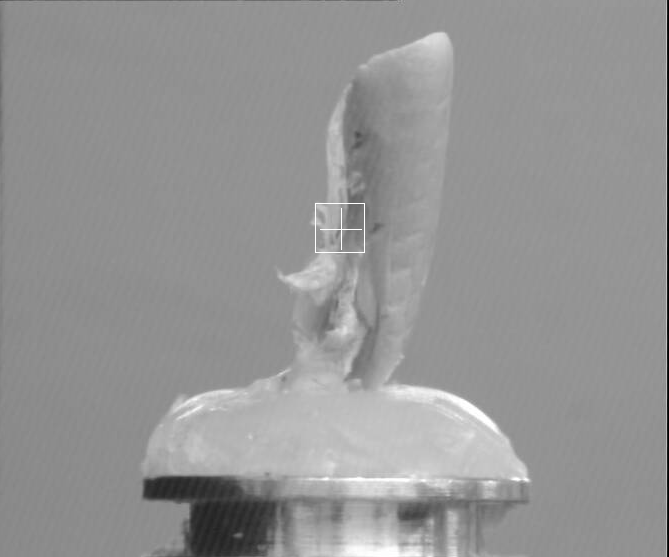
\includegraphics[width=\textwidth]{gfx/lung-paper-figures/KO202_LL_control_1_00degree.png}
    \caption{}
    \label{fig:reconstructed}
    \end{subfigure}
    \hfill
    \begin{subfigure}[b]{.49\textwidth}
    \centering
    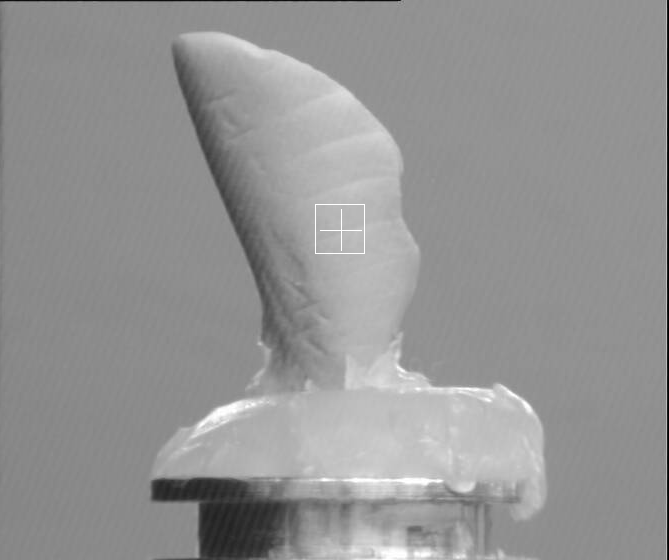
\includegraphics[width=\textwidth]{gfx/lung-paper-figures/KO202_LL_control_1_90degree.png}
    \caption{}
    \label{fig:lung-alignment}
    \end{subfigure}
    \caption[Alignment for lung microtomography.]{Alignment positions
    for the microtomography of the sample labelled KO202. These are recorded
just before each tomographic scan in order to mark the exact location of the
scan itself. This is then relevant to gather data from the radiography on
the Talbot-Lau interferometer on the same area.}
\end{figure}

\subsection{Processing of the synchrotron tomographic data}\label{sec:tomoprocessing}
The tomographic sinograms are preprocessed with the Paganin
algorithm~\parencite{Paganin_2002} and
the 3D volume is then reconstructed with the gridrec
algorithm~\parencite{Marone:pp5022}. The volumes, shown in
figure~\ref{fig:reconstructed} are then thresholded with the Otsu
algorithm~\parencite{Otsu_1979}, with independent thresholds for each slice, to
provide a binary labelling for tissue and air. A cycle of
erosion and dilation is applied to remove single pixel artifacts while still
keeping the septa between neighboring alveoli (figure~\ref{fig:segmented}).
This preserves the structures in the lung because septa, while possibly
being only one pixel in thickness, are also connected to surrounding tissue.
On the other hand, isolated pixels should be removed as they could affect
the subsequent analysis.

\begin{figure}[htb]
    \centering
    \begin{subfigure}[b]{.49\textwidth}
    \centering
    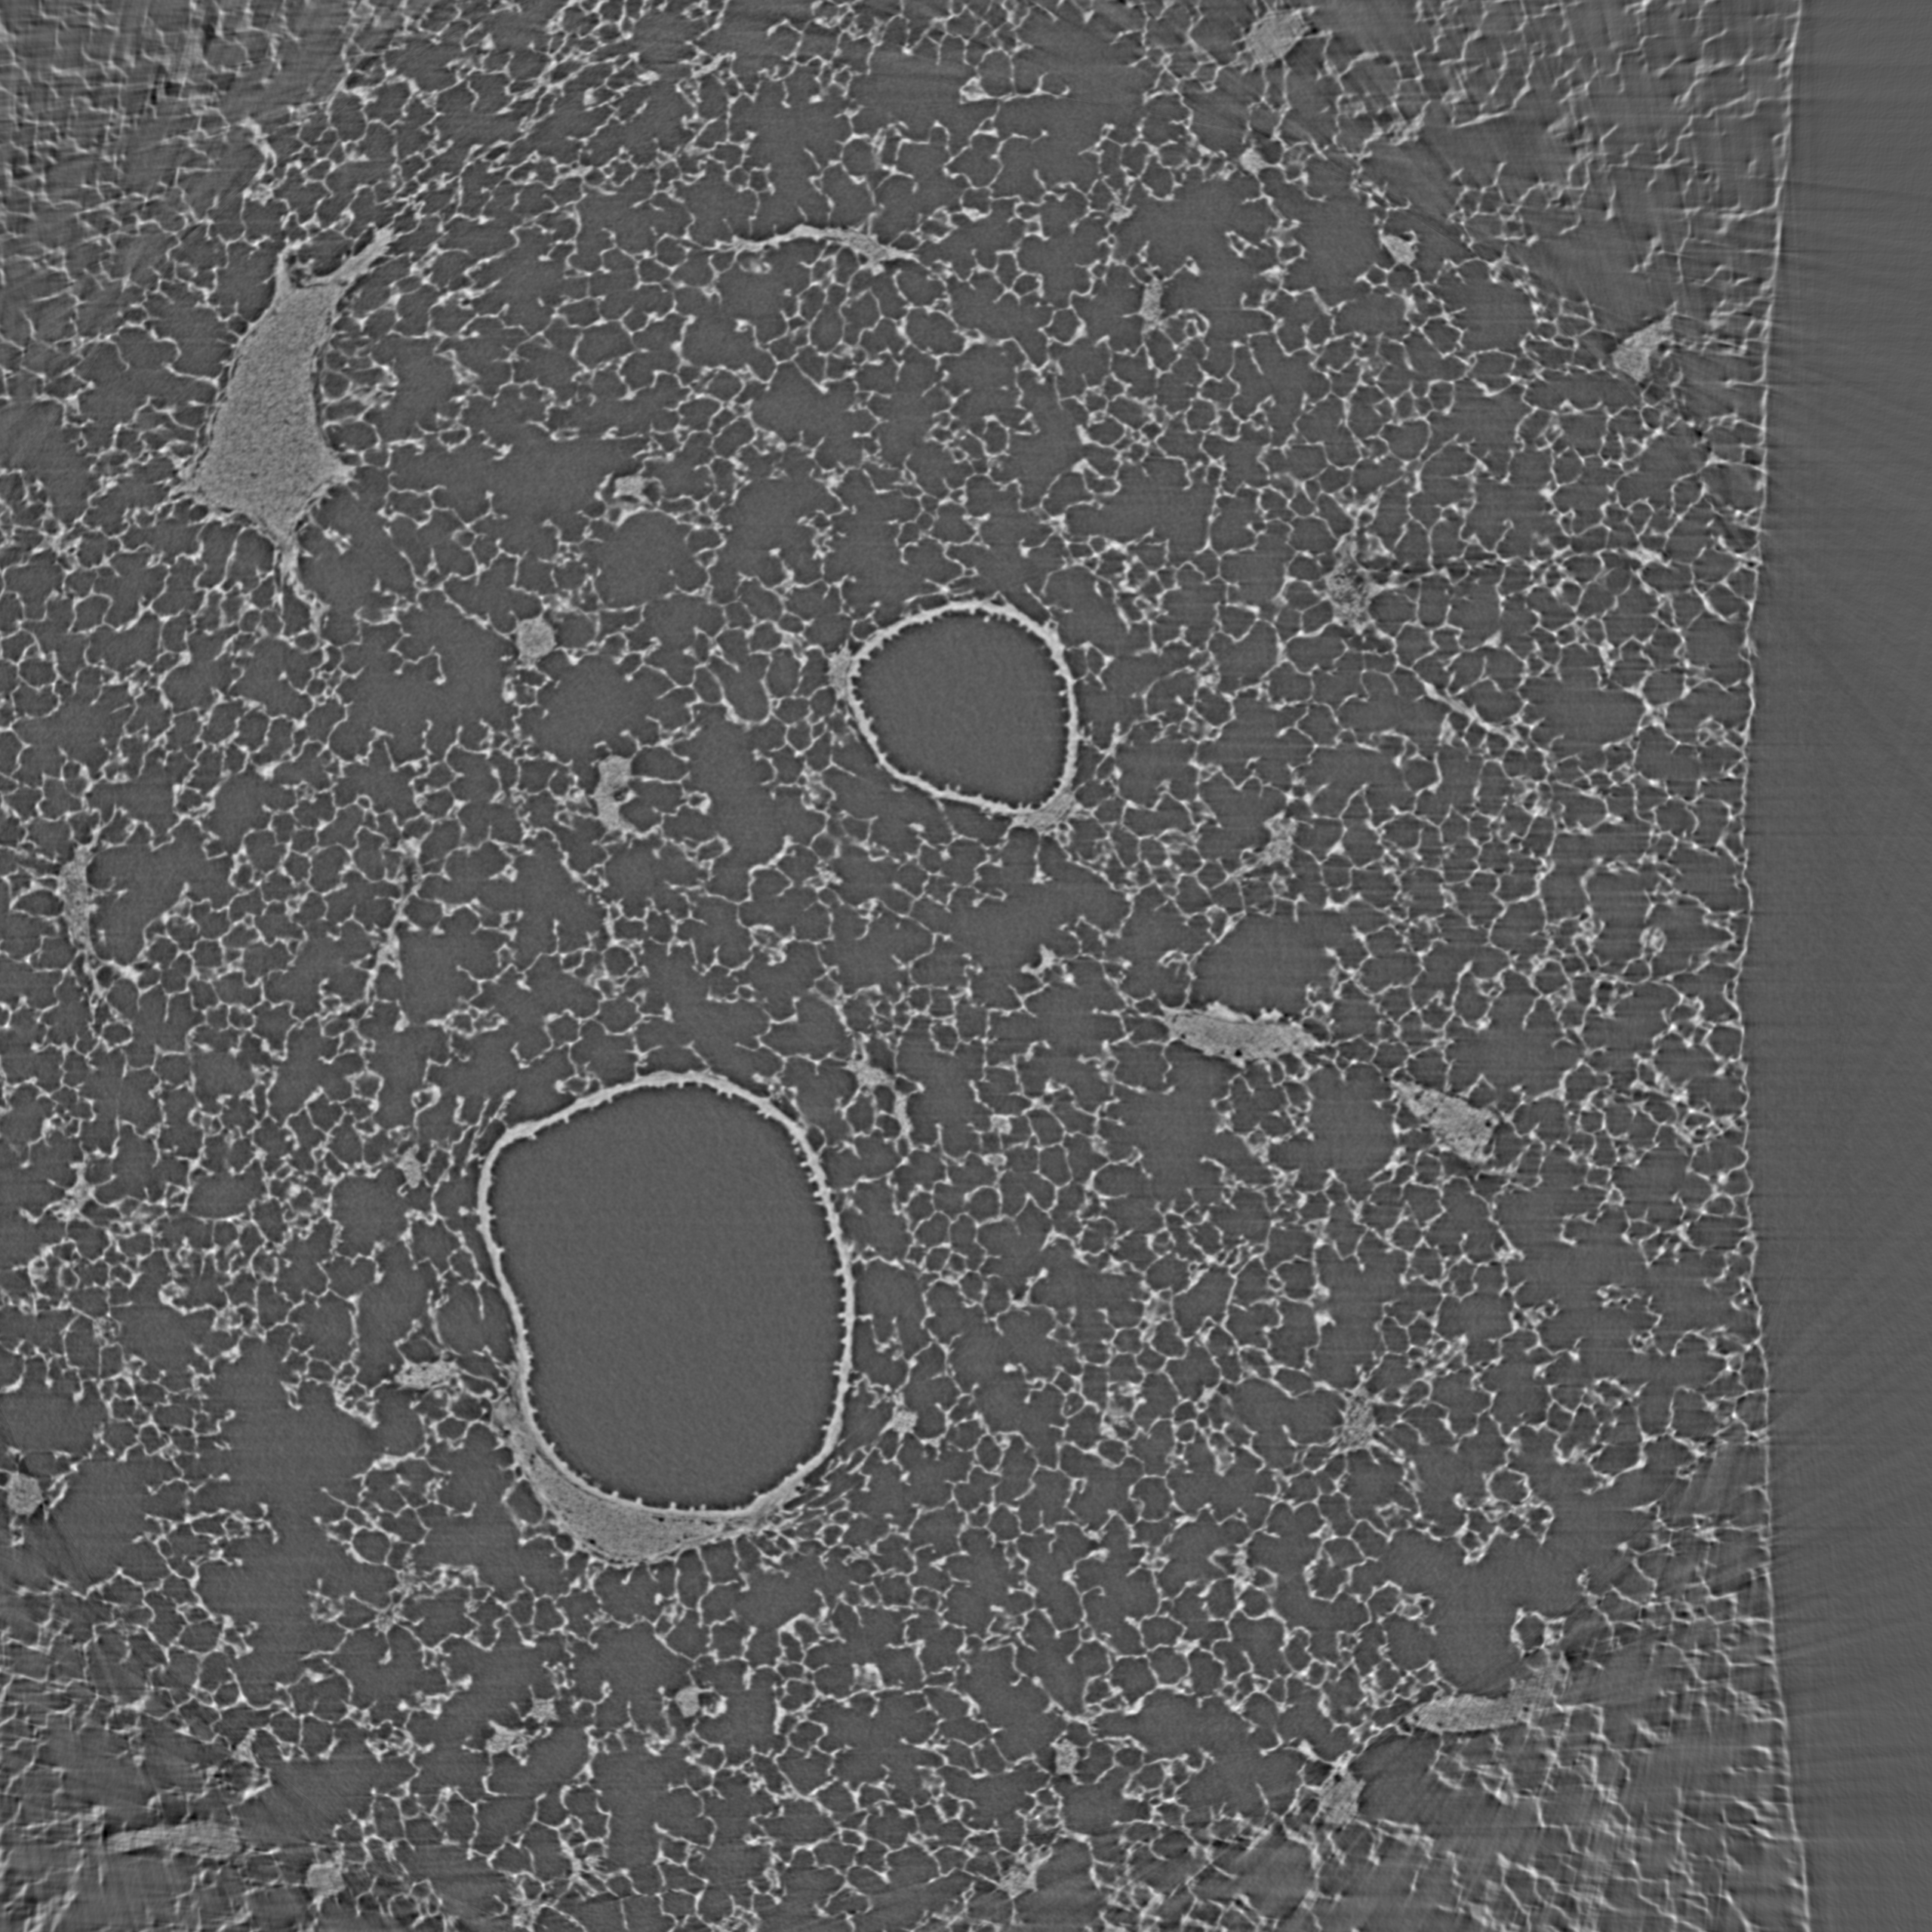
\includegraphics[width=\textwidth]{gfx/lung-paper-figures/KO202_LL_control_20700_rec16bit.png}
    \caption{}
    \label{fig:reconstructed}
    \end{subfigure}
    \hfill
    \begin{subfigure}[b]{.49\textwidth}
    \centering
    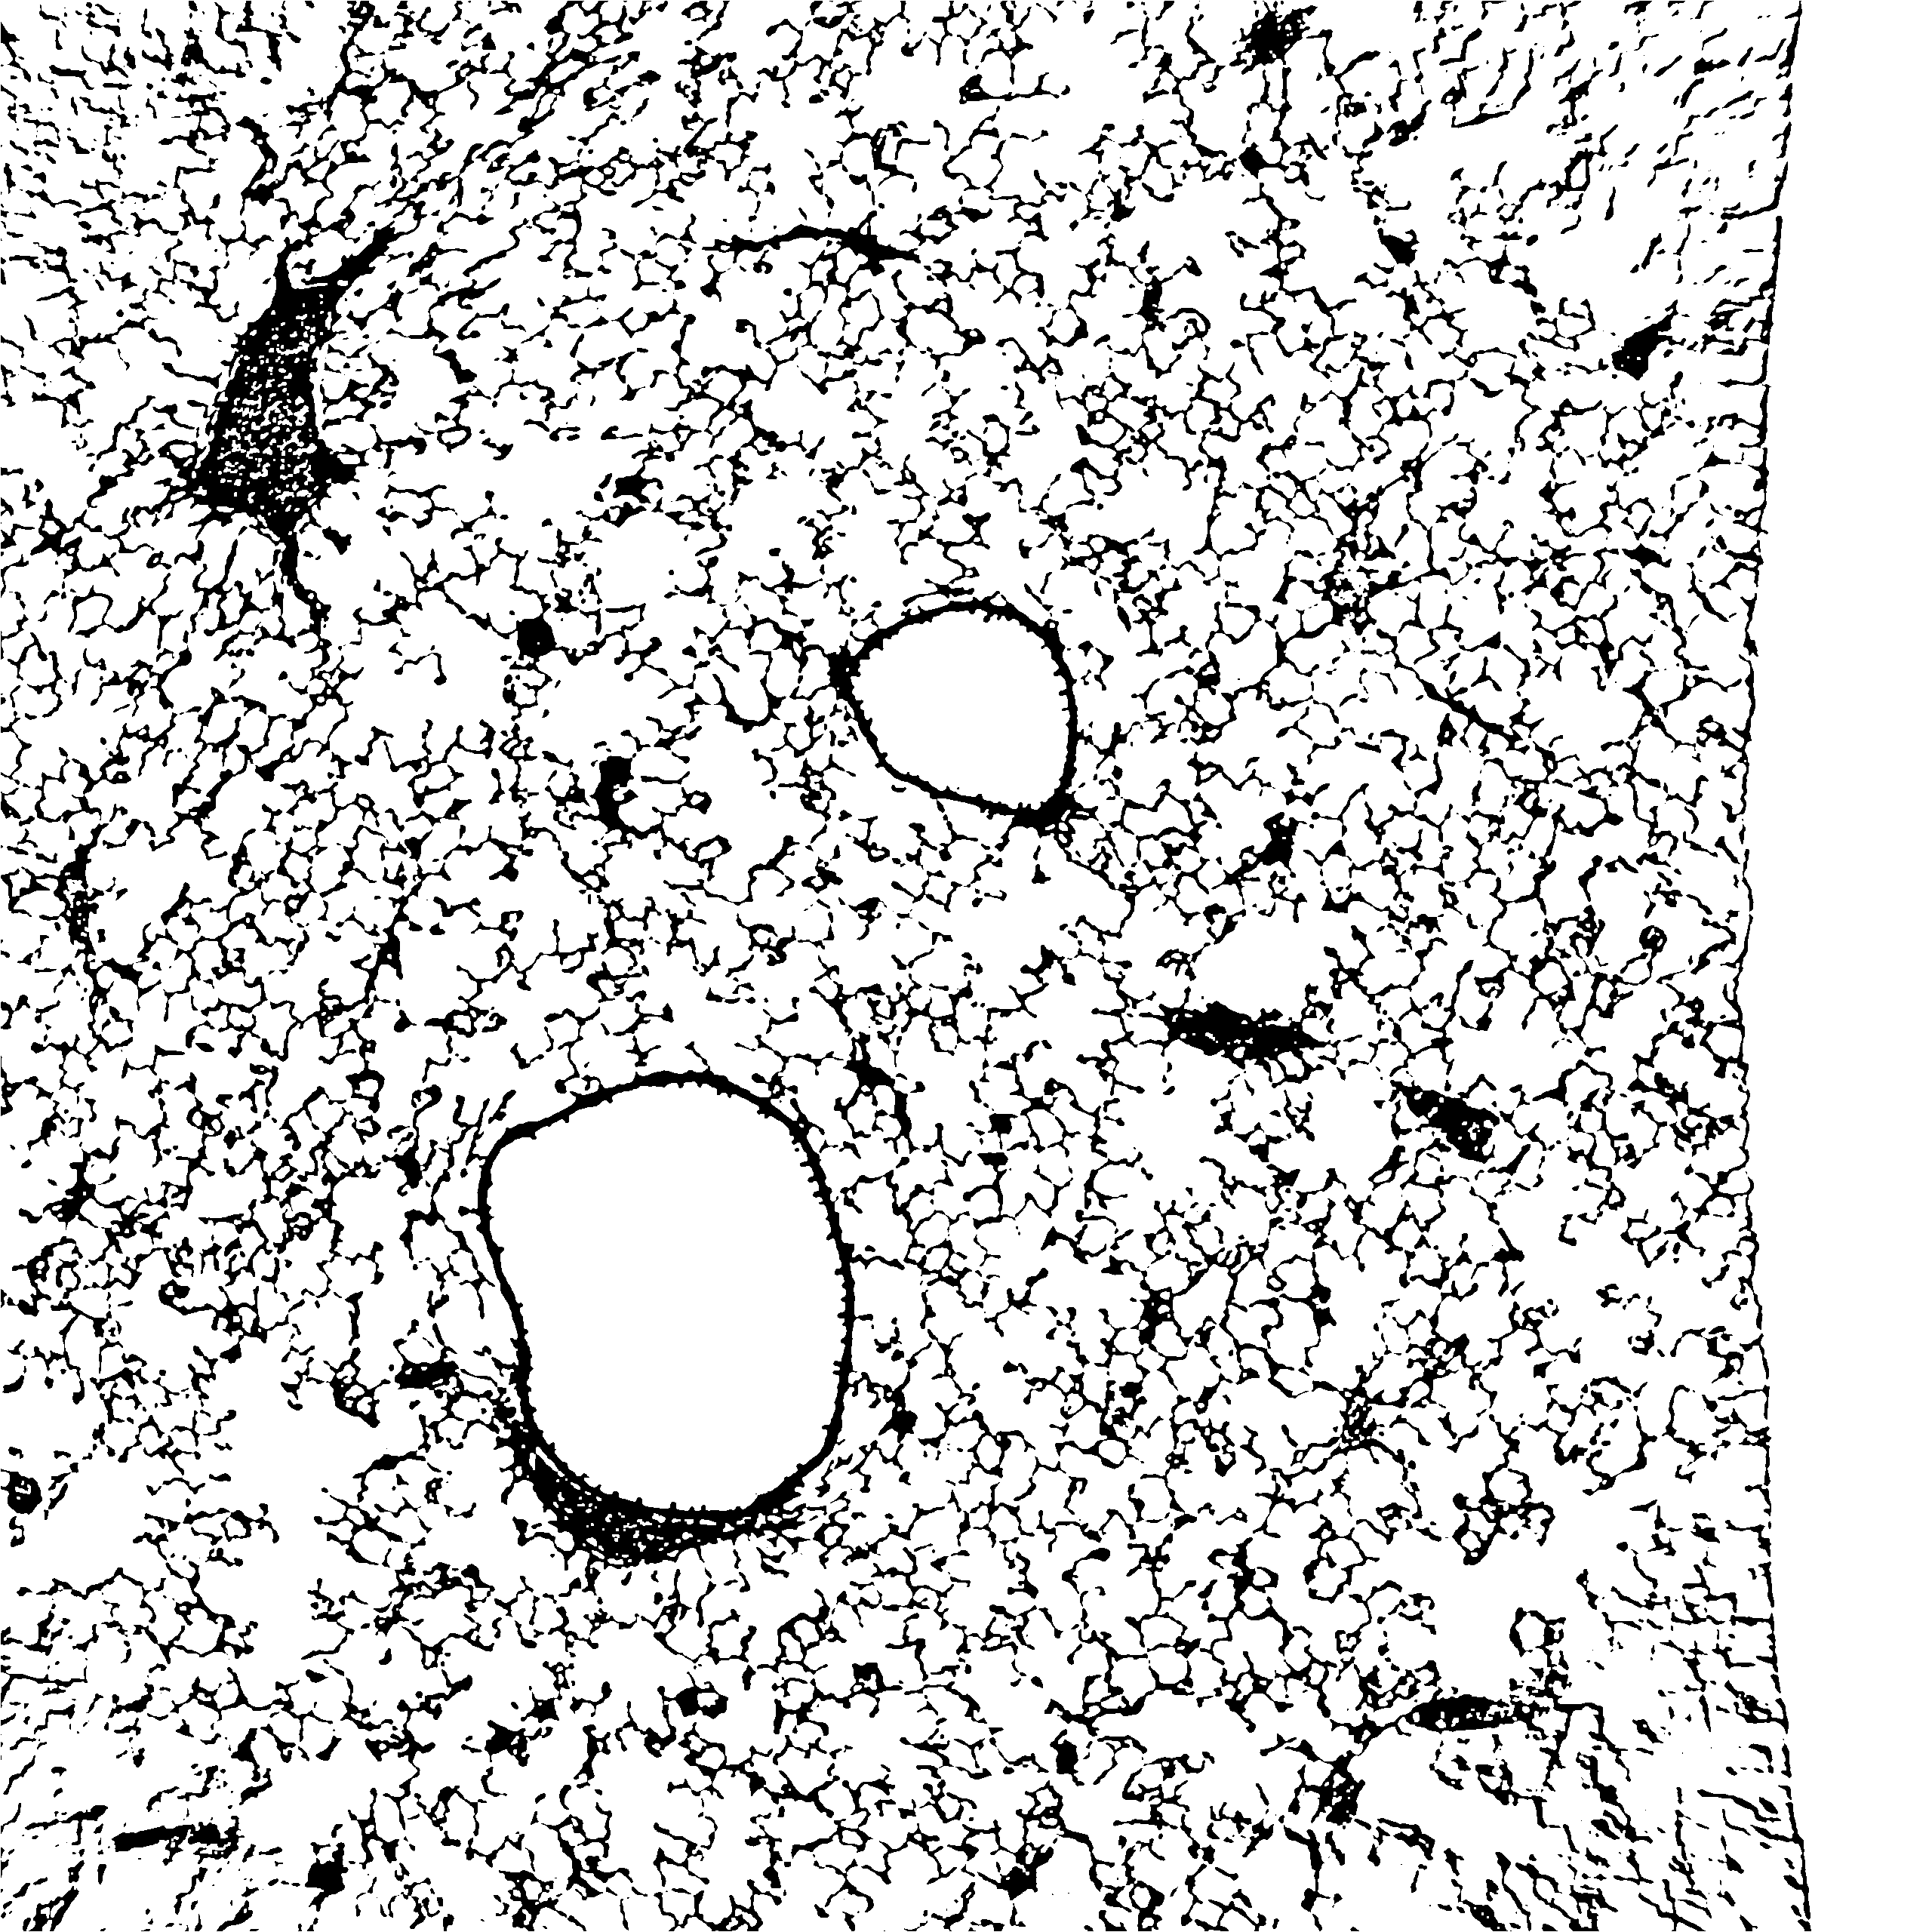
\includegraphics[width=\textwidth]{gfx/lung-paper-figures/rec_16bit_segmented0700_compressed.png}
    \caption{}
    \label{fig:segmented}
    \end{subfigure}
    \caption[Reconstruction of a lung microtomography.]{Reconstruction
        (left) and
        segmentation (right) of a local microtomography of the sample KO202,
        performed at the X02DA TOMCAT beamline.}
\end{figure}

Next, each lung sample is manually stitched from three or four local
tomographies (figure~\ref{fig:stitched}), depending on the sample thickness, and the local air thickness
map is calculated. The local thickness map is an algorithm developed for
bone analysis or foam analysis in material science~\parencite{localthickness}, that aims
at calculating the maximum diameter of a sphere fitting in each hole in the
sample.
\begin{figure}[htb]
    \centering
    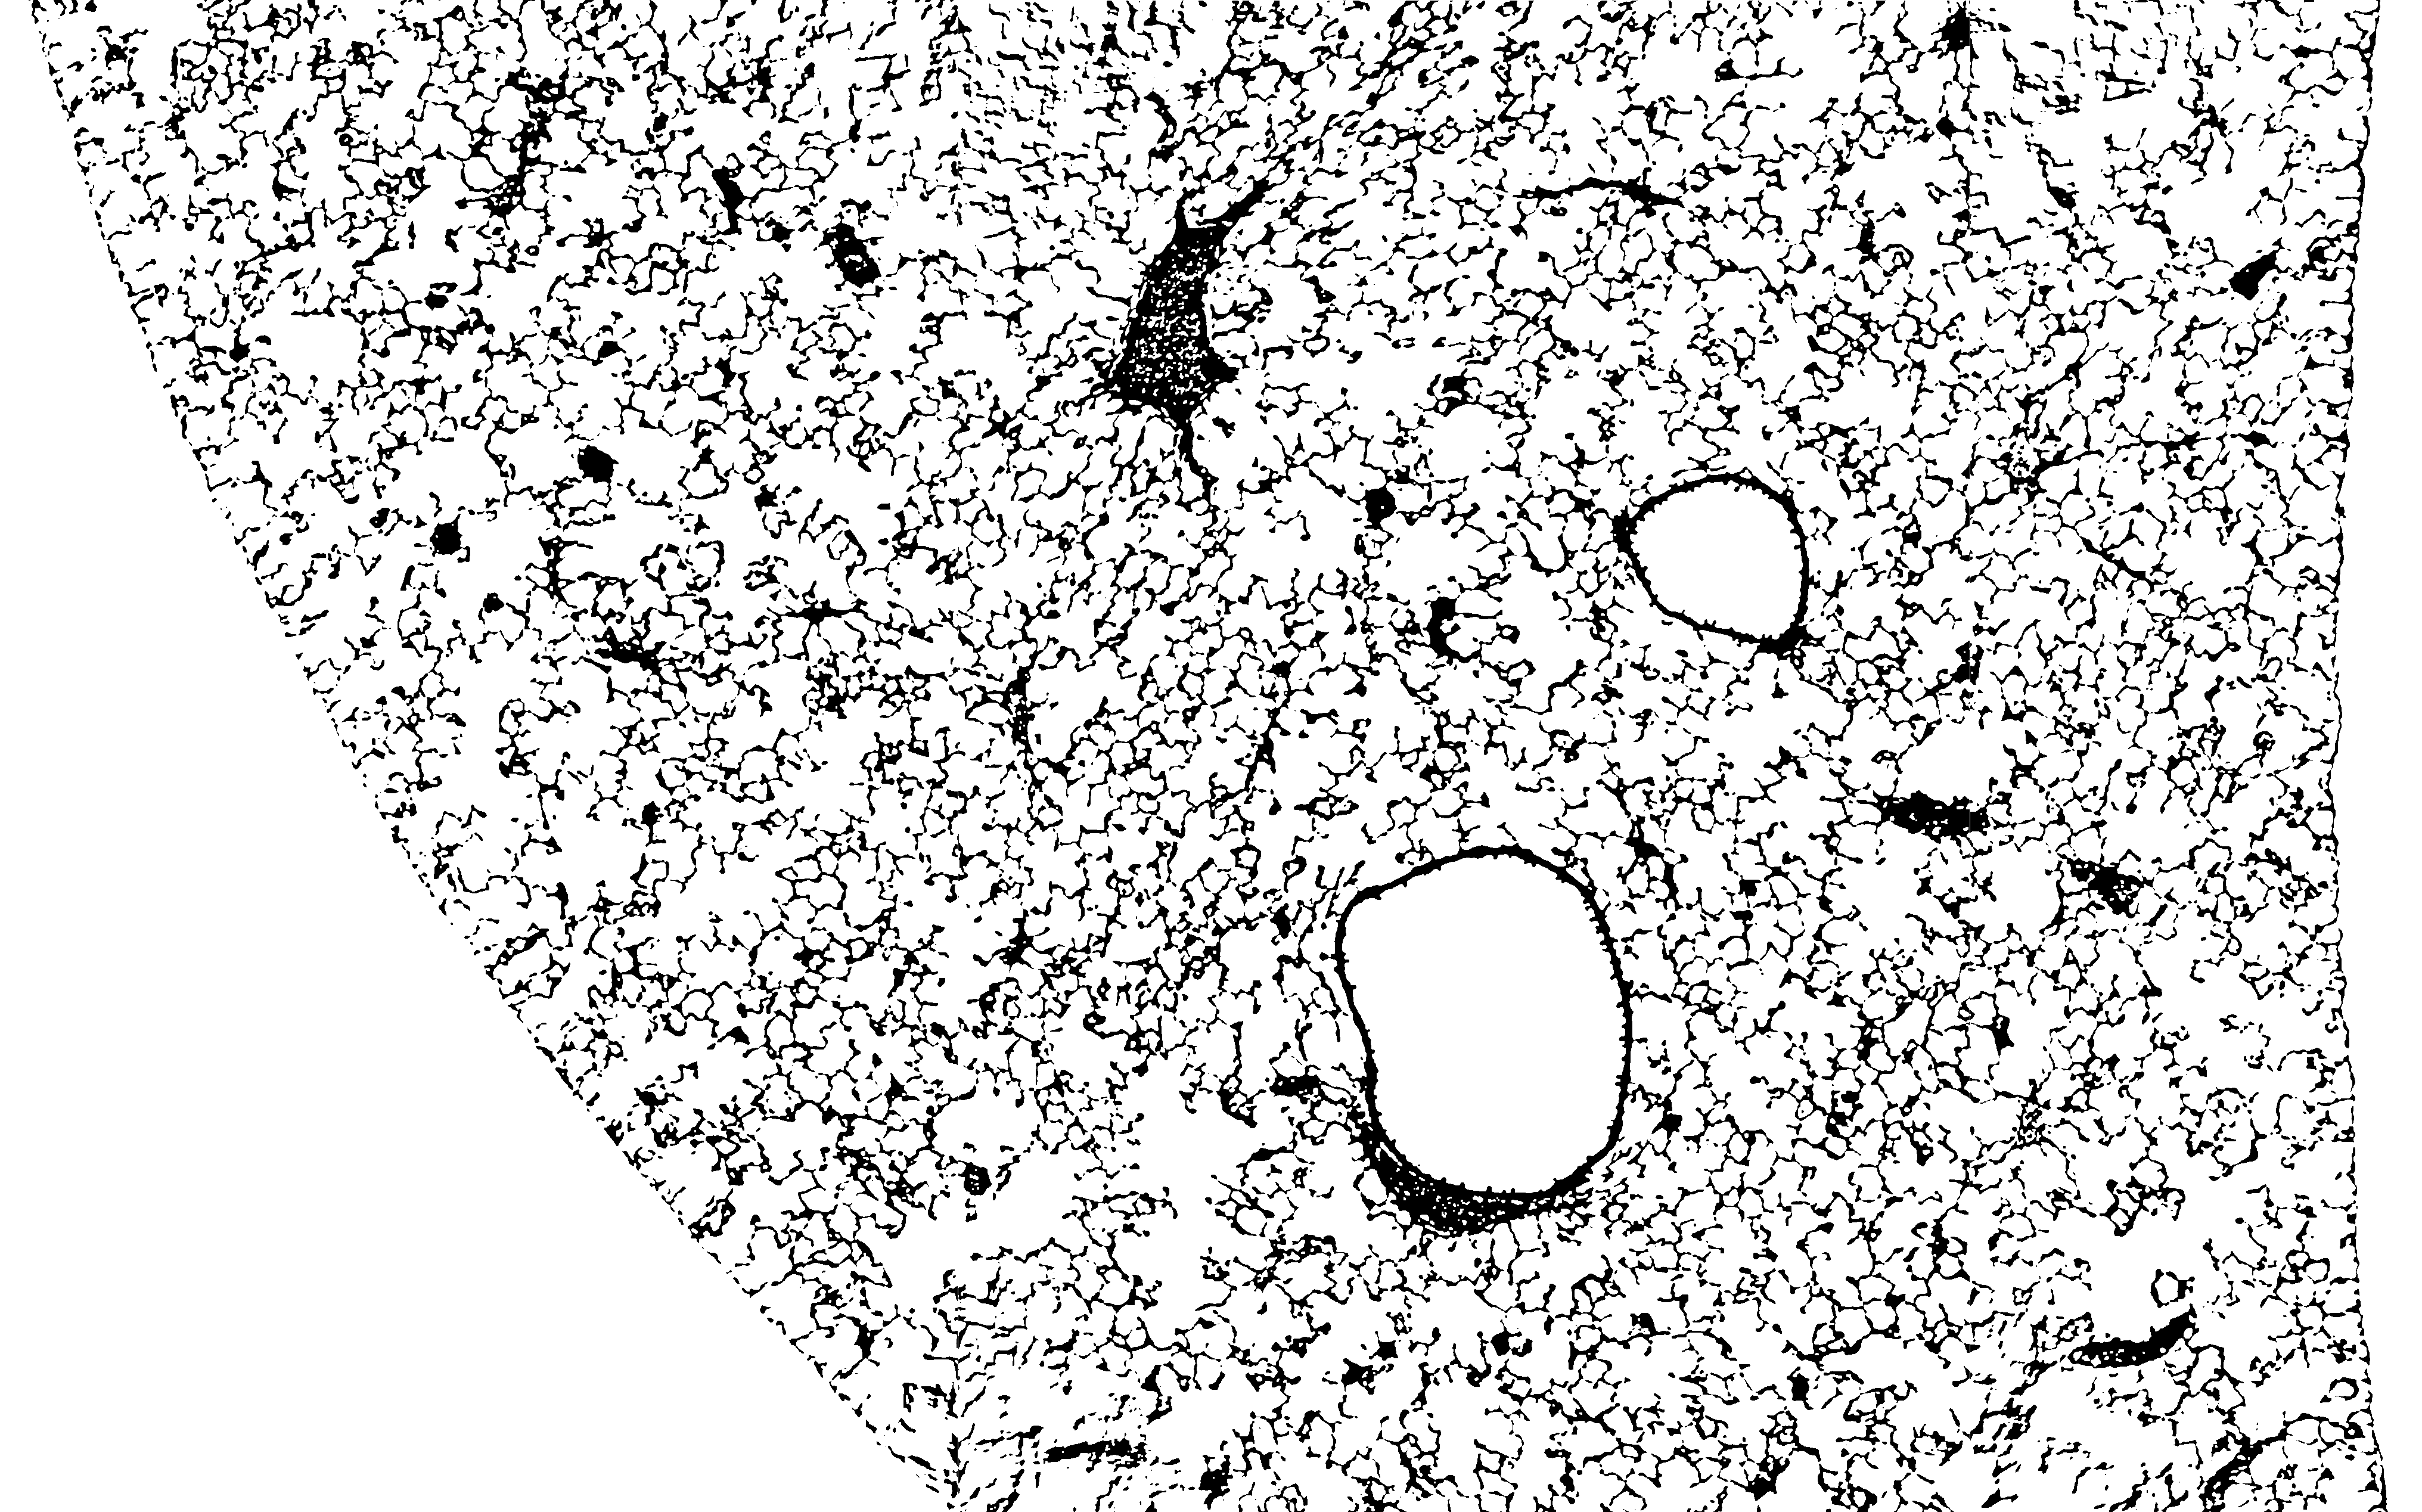
\includegraphics[width=\textwidth]{gfx/lung-paper-figures/0700.png}
    \caption[Stitched beamline tomography of a mouse lung.]{Stitched slice of the mouse lung labelled KO202, measured on
    the X02DA TOMCAT beamline.}
    \label{fig:stitched}
\end{figure}
The euclidean distance transform is calculated from the image, yielding the
distance of each point in the airways from the closest
wall (figure~\ref{fig:distance-ridge}).
\begin{figure}[htb]
    \centering
    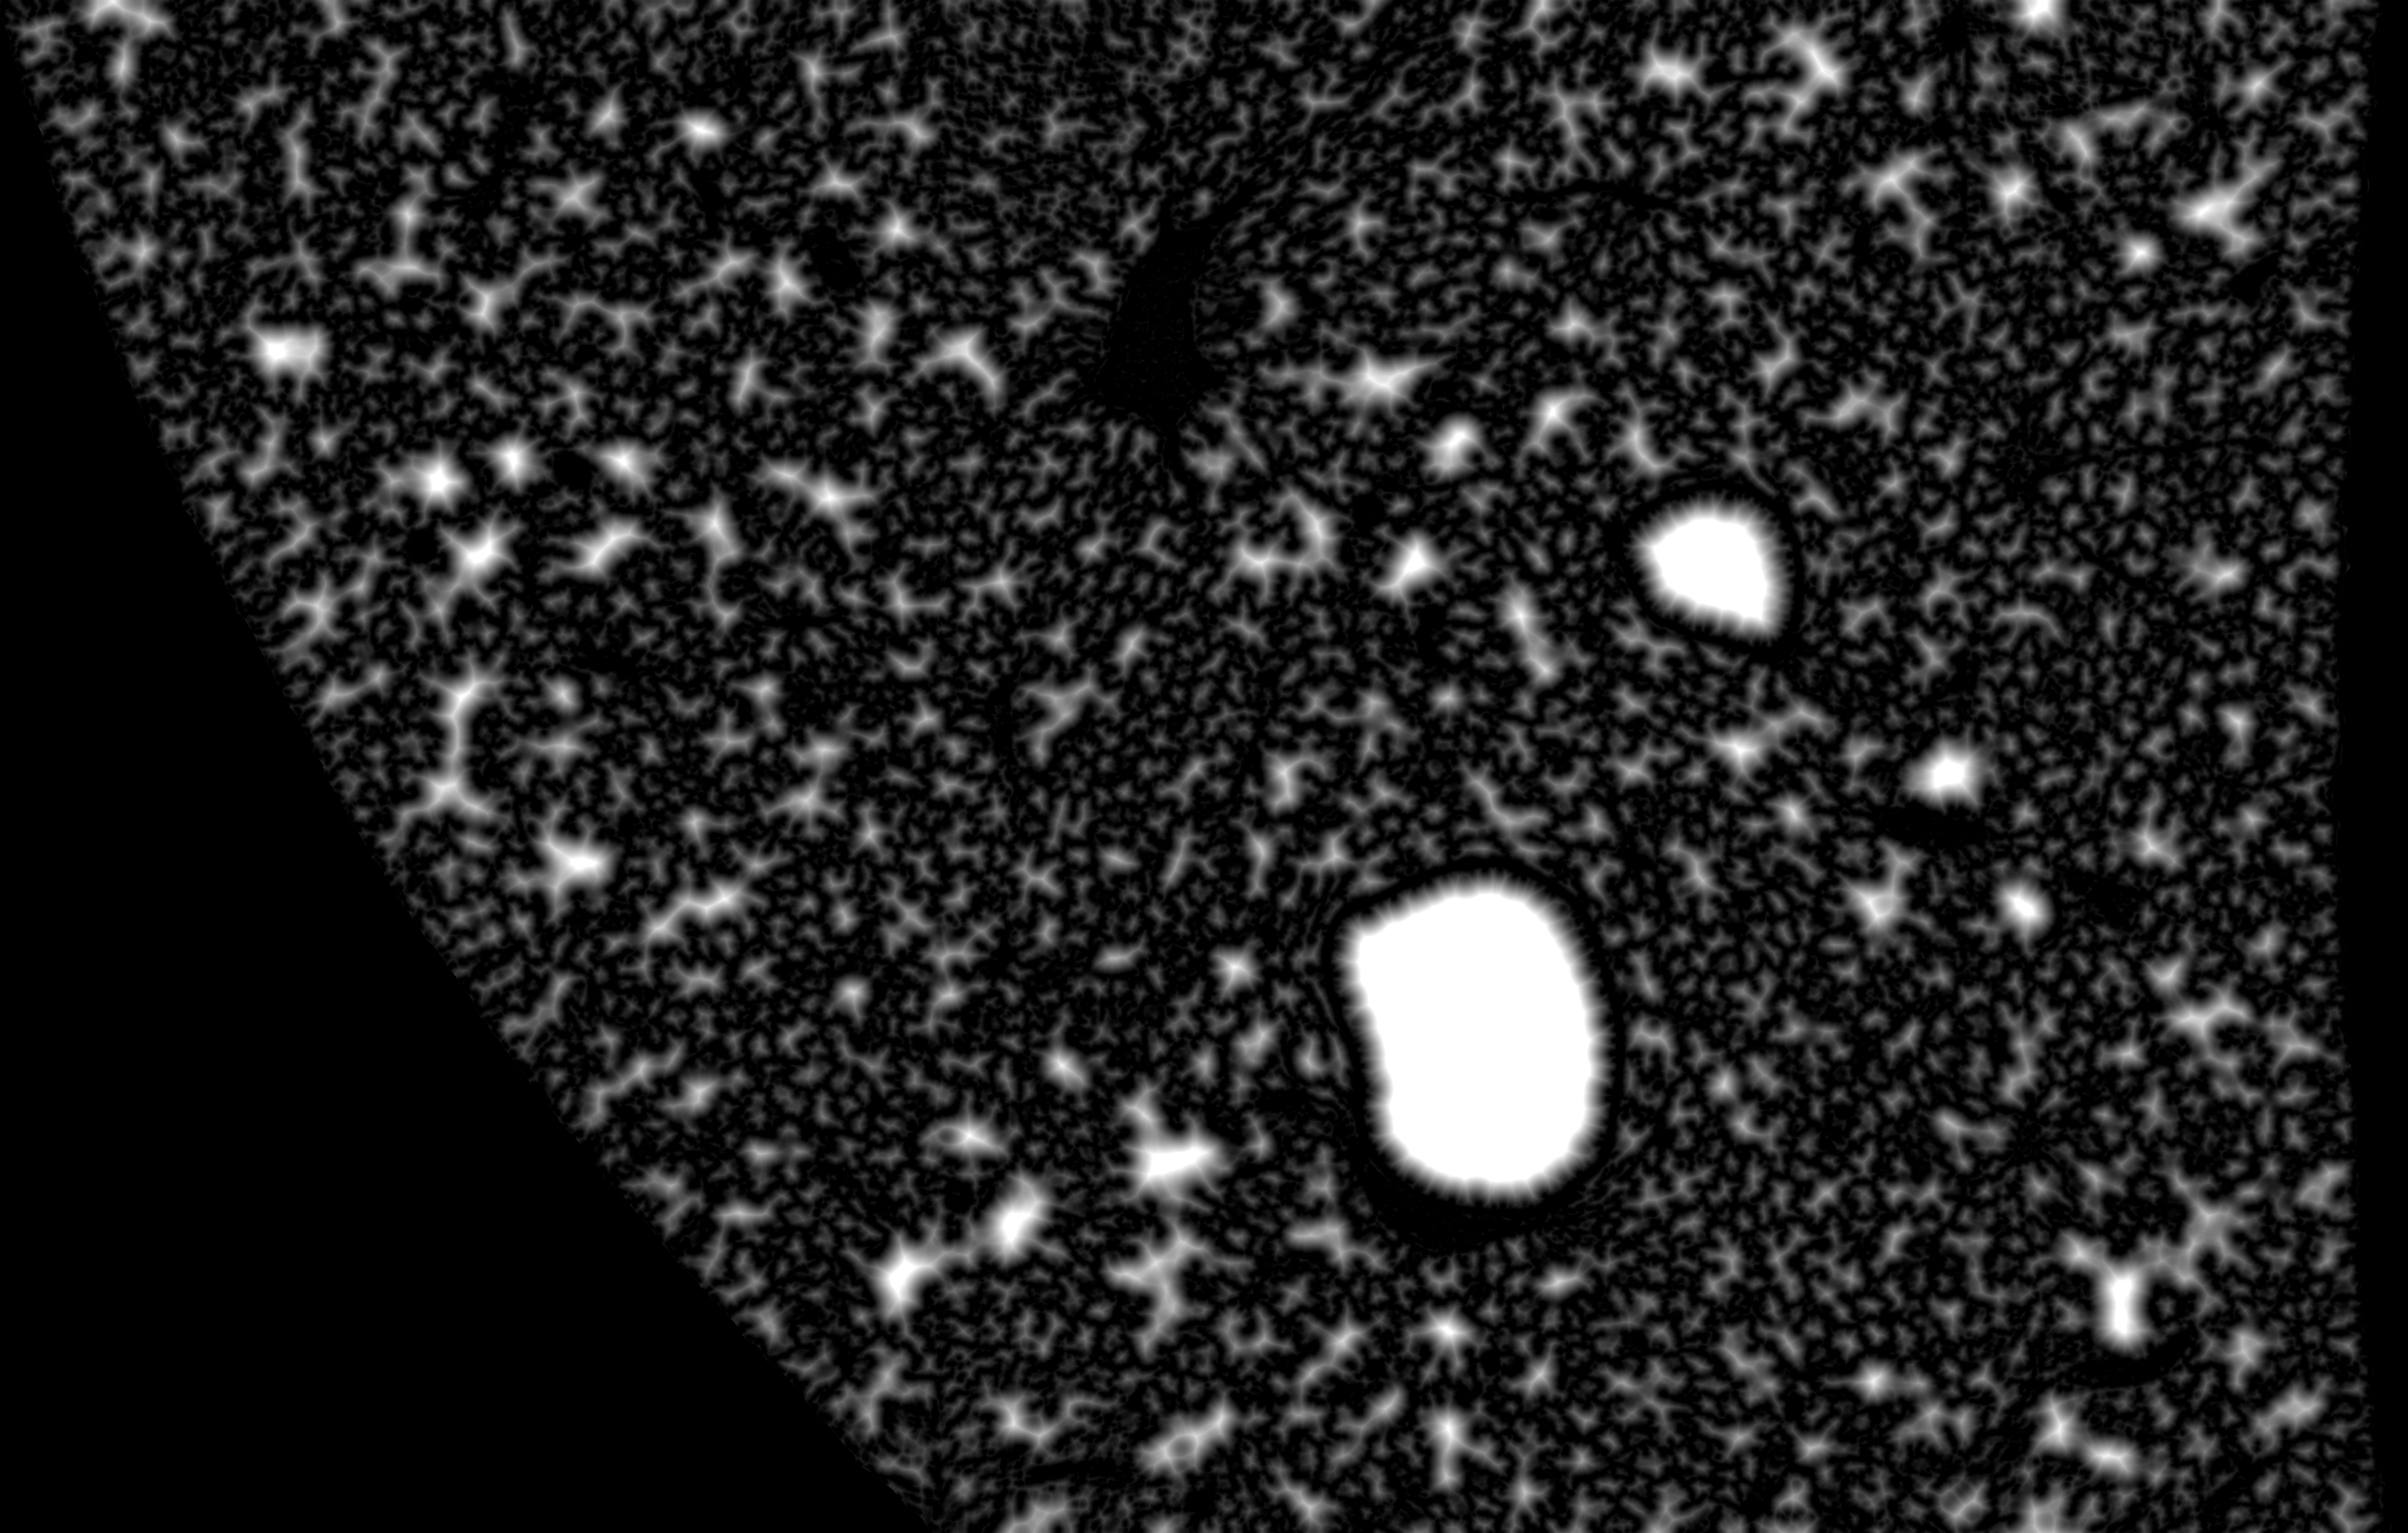
\includegraphics[width=\textwidth]{gfx/lung-paper-figures/KO202_DR_700.png}
    \caption[Euclidean distance transform.]{Euclidean distance transform of figure~\ref{fig:stitched},
where each pixel encodes its distance from the closest wall. Sample with
label KO202.}
    \label{fig:distance-ridge}
\end{figure}
The points in the transformed dataset are then sorted in descending order in
order to fit the largest possible sphere at each location.

In the case of lungs, each of the airways is filled with the largest possible
sphere, resulting in a model where the lung airways are a collection of
spheres embedded in the background of the tissue
(figure~\ref{fig:thickness-map}).
\begin{figure}[htb]
    \centering
    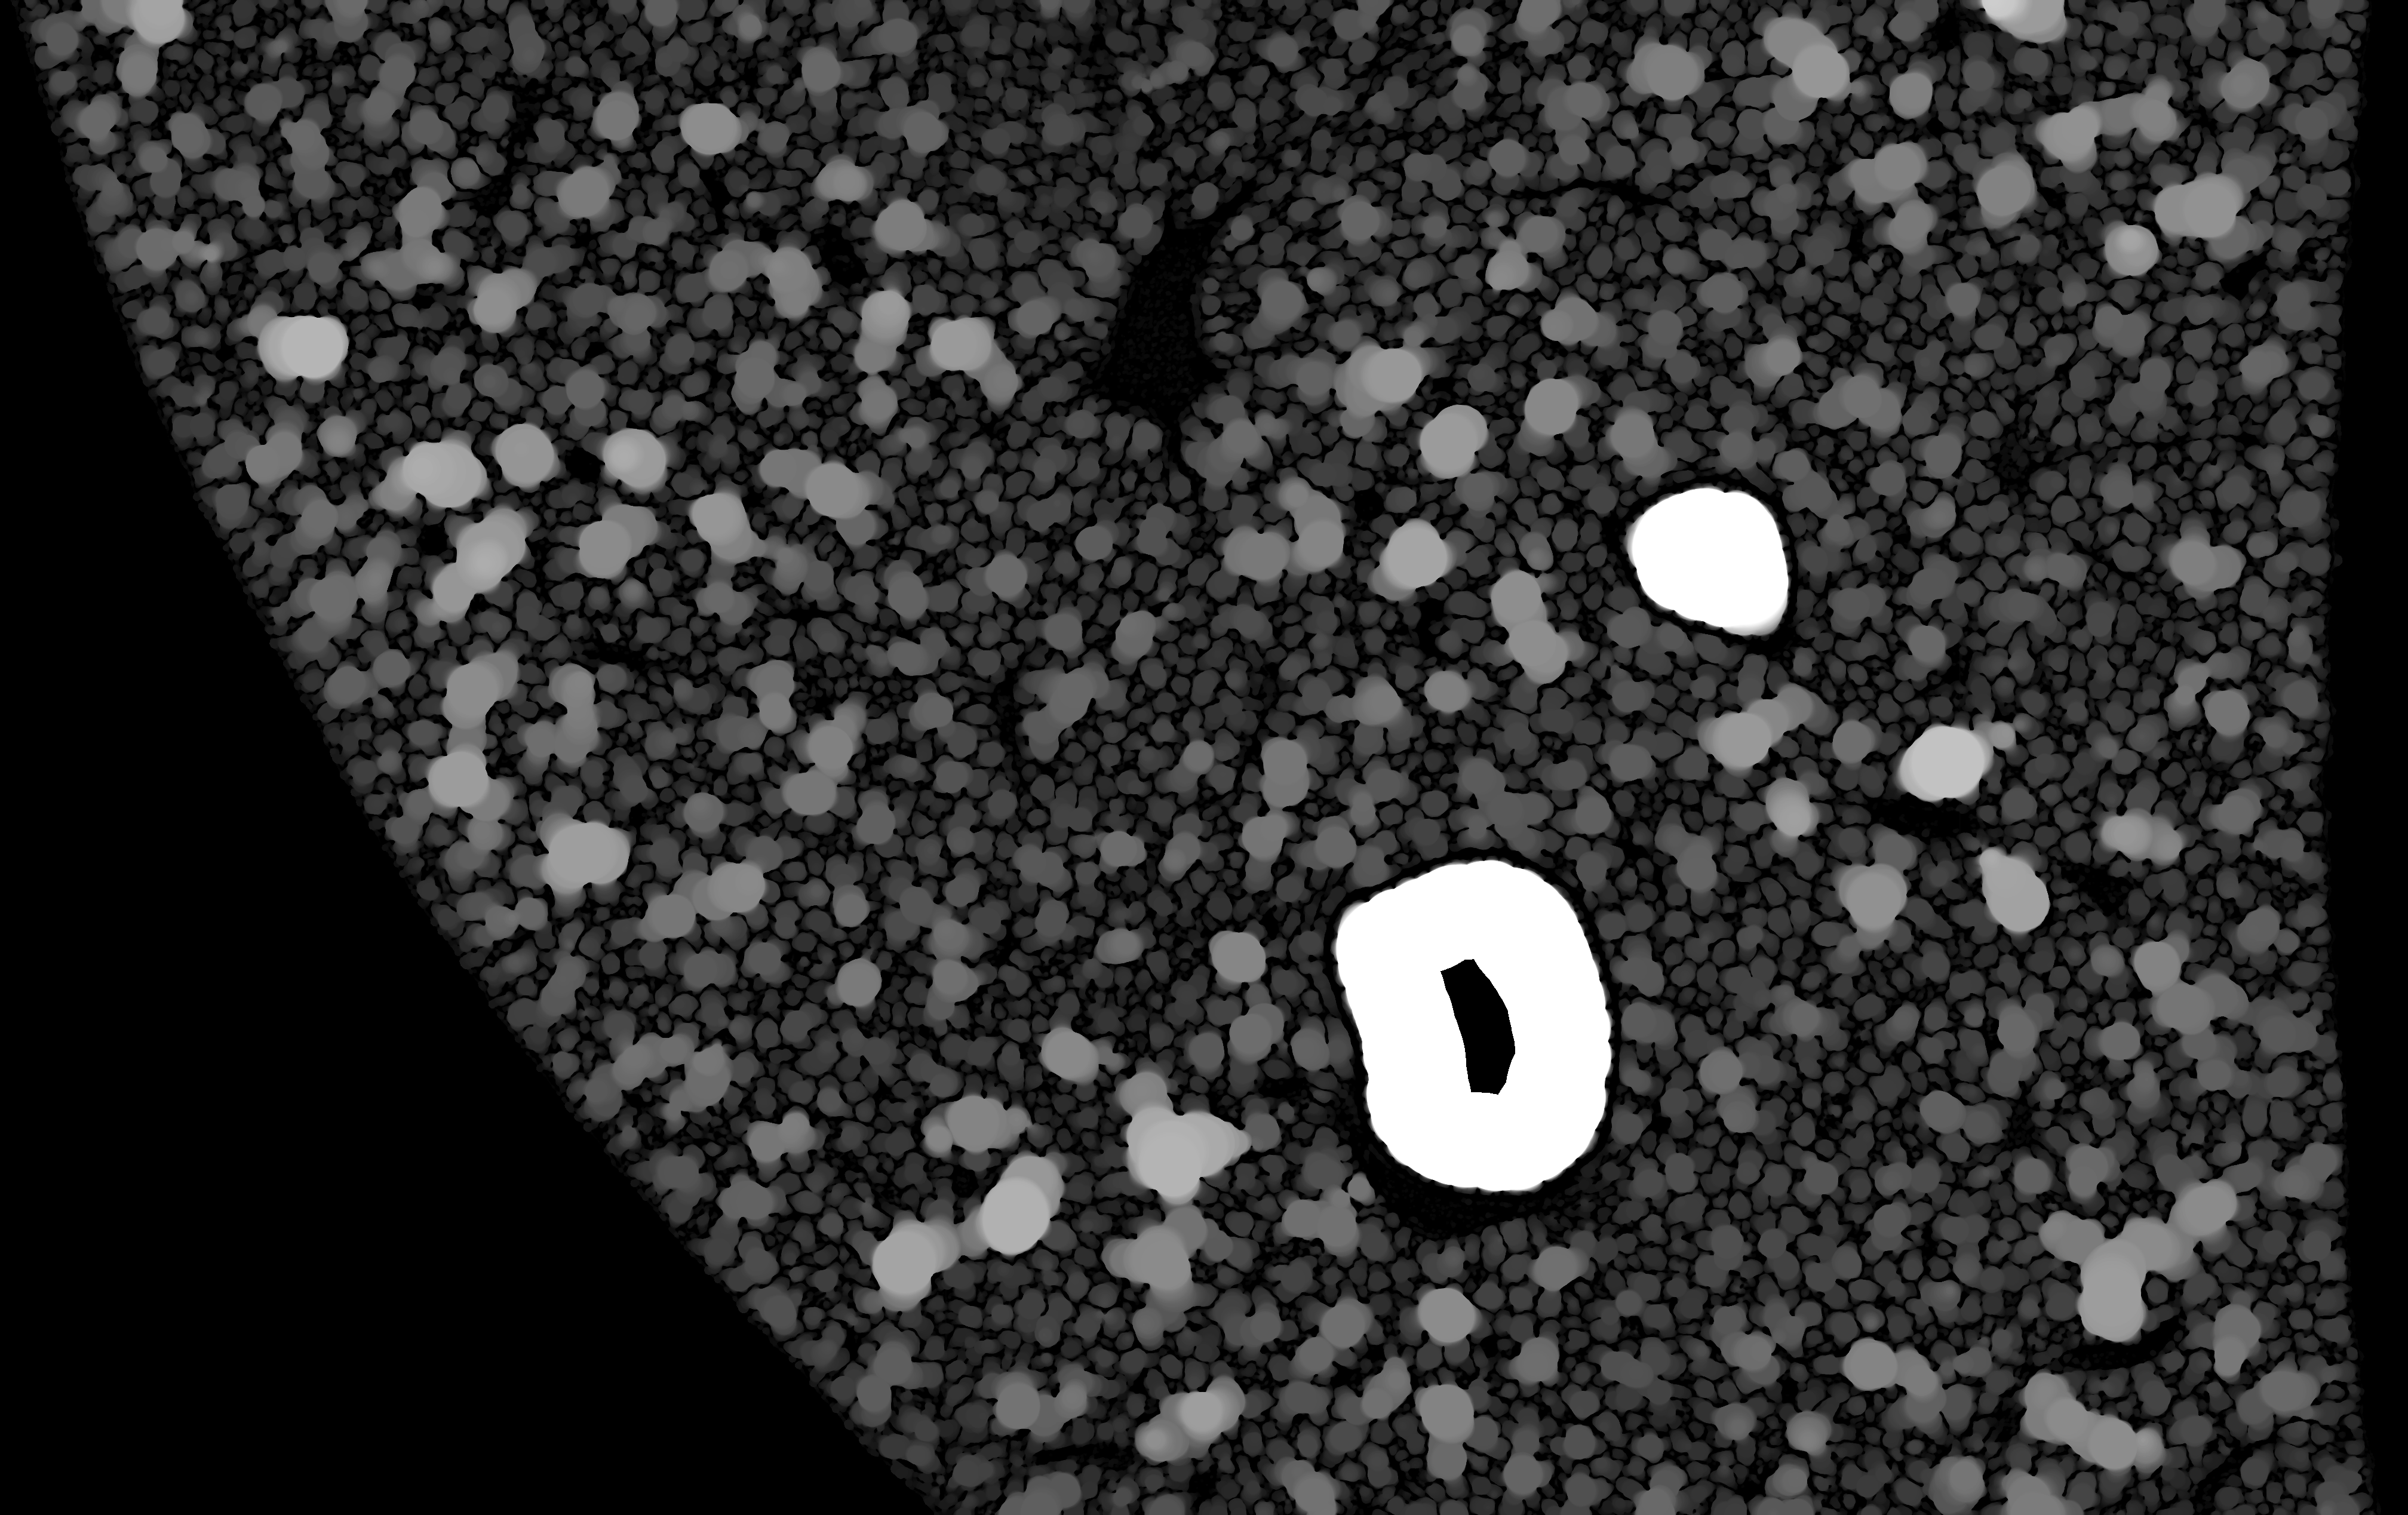
\includegraphics[width=\textwidth]{gfx/lung-paper-figures/KO202_TM_700.png}
    \caption[Local thickness map.]{Thickness map of
        figure~\ref{fig:distance-ridge}. Airways are filled with spheres
        with the largest diameter that fits between the walls. These
        diameter distribution is then used to produce
        figure~\ref{fig:sizepdf}.}
    \label{fig:thickness-map}
\end{figure}
To obtain a distribution of sphere sizes, kernel density estimation in the R
statistics package \emph{ks}~\parencite{JSSv021i07} is used in order to avoid possible artifacts
resulting from the arbitrary binning of the histogram of sphere sizes.

\subsection{Processing of the radiographic data from the laboratory source}\label{sec:radioprocessing}
For each pixel, the transmission image $A$ and the
dark-field image $B$ are calculated (see fig.~\ref{590406}). Both of these
quantities are known to follow the Beer-Lambert law, with an exponential
decay related to the thickness $t$ of the sample: $A = \exp(-\mu_A t)$, $B =
\exp(-\mu_B t)$. Since the lung samples are irregular in shape, it is
beneficial to examine the ratio of the logarithms $R$ in
order to remove the local dependence on the thickness of the sample in the
radiography:
\begin{align}
    A &= \dfrac{a_{0,s}}{a_{0,f}}\\
    B &= \dfrac{a_{1,s}}{a_{1,f}}\dfrac{a_{0,f}}{a_{0,s}}\\
    R &= \dfrac{\log(B)}{\log(A)}.
    \label{eqn:definitions}
\end{align}
\begin{figure}[h!]
    \centering
    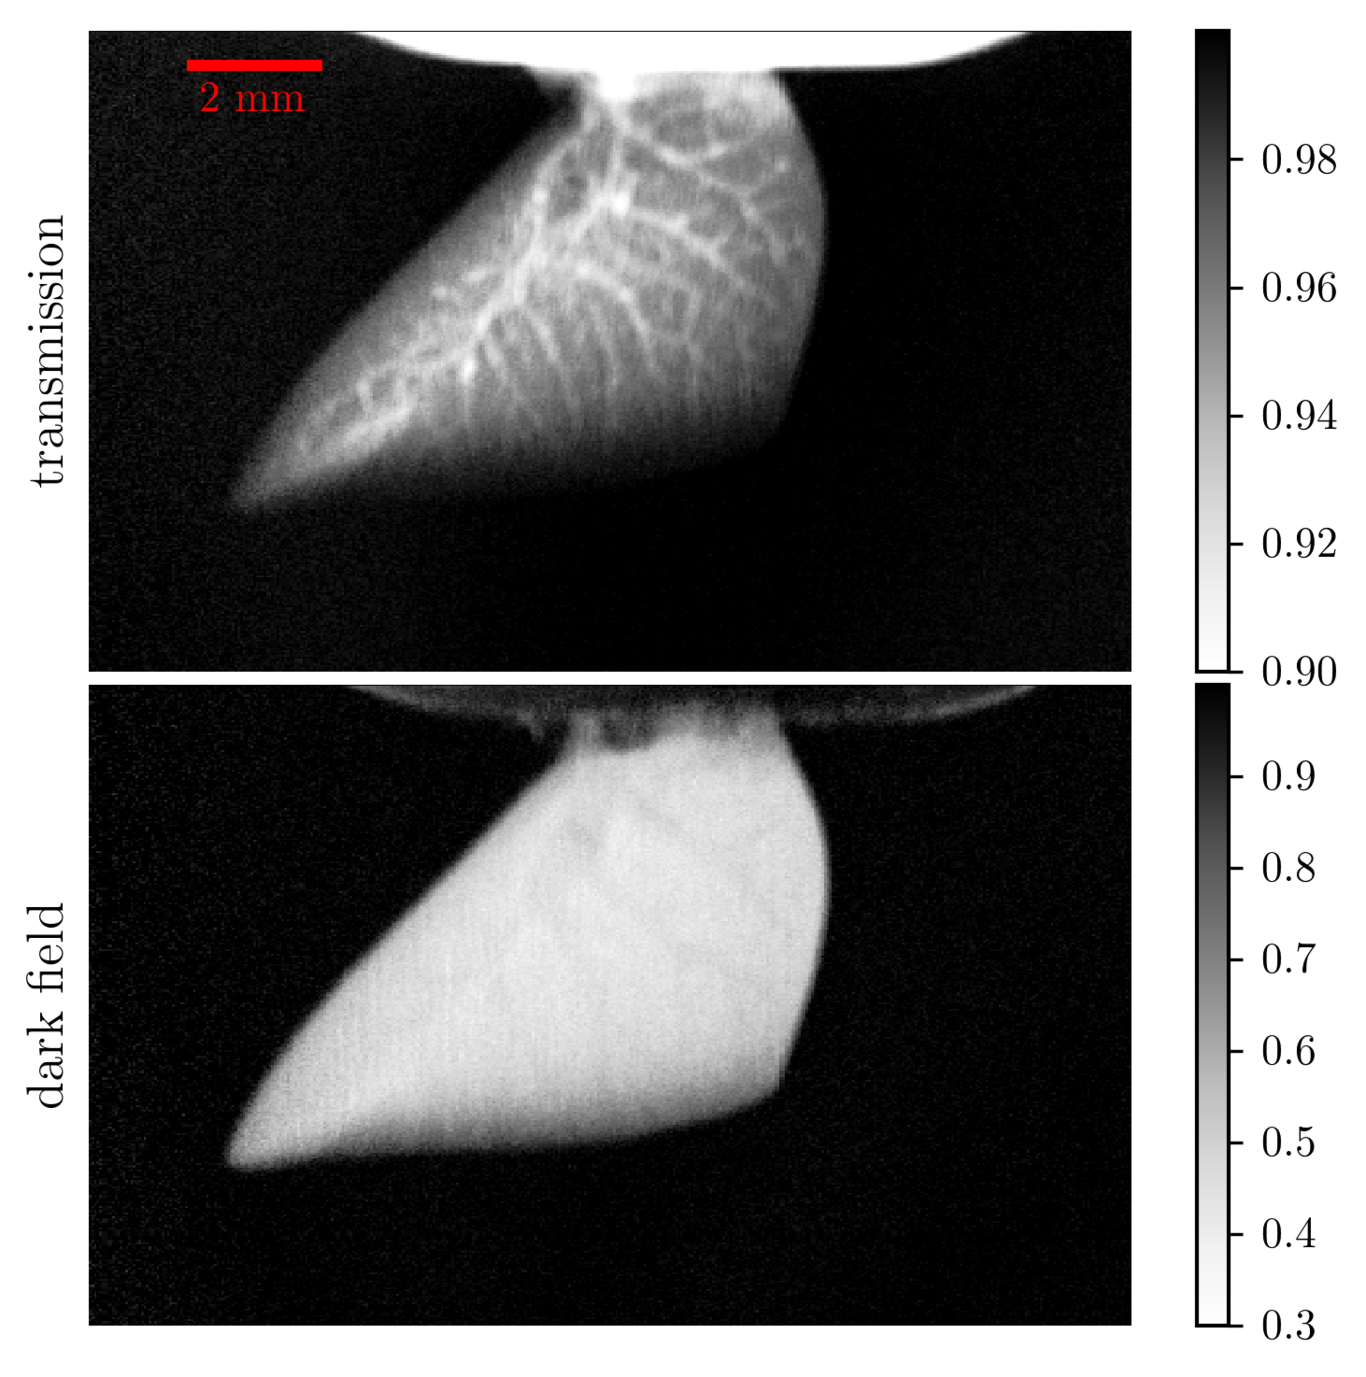
\includegraphics[width=0.70\columnwidth]{gfx/lung-paper-figures/KO373_LL_smoke/WT256_LL_smoke}
    \caption[Radiography of a mouse lung on a laboratory source]{Example of an ex vivo lung interferometric radiography on a laboratory
        source. Sample labelled WT256.
        {\label{590406}}}
\end{figure}

\section{Modelling the polychromatic dark-field signal}\label{sec:model}
Previous works~\parencite{Lynch:11,Gkoumas2016} have demonstrated quantitative estimation of
the dark-field signal for a monochromatic source and monodisperse solutions
of micrometer-sized spheres. In particular, the coefficient $\mu_B$, for a
beam of wavelength $\lambda$ is:
\begin{equation}
\mu_B = \frac{3\pi}{\lambda^2}f |\Delta n|^2 d
    \begin{cases}
    D' & \text{if } D' \leq 1\\
    \begin{aligned}
    & D' - \sqrt{D'^2 - 1}\\
    & (1 + D'^{-2}/2) \\
    & + (D'^{-1} + D'^{-3} / 4) \\
    & \log\left(\frac{D' + \sqrt{D'^2 - 1}}{D' - \sqrt{D'^2 - 1}}\right)
    \end{aligned} & \text{otherwise.}
    \end{cases}\label{eqn:lynch}
\end{equation}

The autocorrelation length is $d = L\lambda / p$ with $L$ the sample to
detector distance, $p$ and the period of $G_2$. $D'$ is a normalized
particle diameter equal to $D/d$, where $D$ is the particle diameter. $f$ is
the fraction of volume occupied by the scattering material and $n = 1 -
\delta - i\beta$ is the complex refractive index.

We rewrite this formula more concisely as
\begin{equation}
    \mu_B(\energy) = C |\Delta n(\energy)|^2 \energy u(\energy),
    \label{eqn:lynchshort}
\end{equation}
where $\energy$ is the energy of the beam, $C = 3 fL / 4p$ is a constant
depending only on the setup geometry and the volume fraction $f$ occupied by
the spheres and $\energy$ is the energy of the beam.

In the case of a polychromatic source, we tested a model where different
energies interact with the sample independently of each other, thus allowing
an incoherent sum of the dark-field signals over the spectral weights
$s(\energy)$:
\begin{equation}
    R = C \frac{\sum_\energy s(\energy)|\Delta n(\energy)|^2 \energy u(\energy)}{\sum_\energy s(\energy) \energy \beta}.
    \label{eqn:lynchpolychromatic}
\end{equation}

This formula, that we can call the \emph{GI method} (grating interferometry) for the calculation of
the dark-field extinction coefficient (figure~\ref{fig:equivalence-lynch-saxs}), was first tested on monodisperse solution of silicon dioxide
spheres with sizes ranging from \SI{0.166}{\micro\meter} to
\SI{7.760}{\micro\meter}, with a volume fraction of 20\%
in glycerol. This model yields a good agreement between the continuous line
and the experimental data representing radiographies of the silicon dioxide
sphere samples recorded on the laboratory source interferometer (figure~\ref{725462}).
\begin{figure}[h!]
\begin{center}
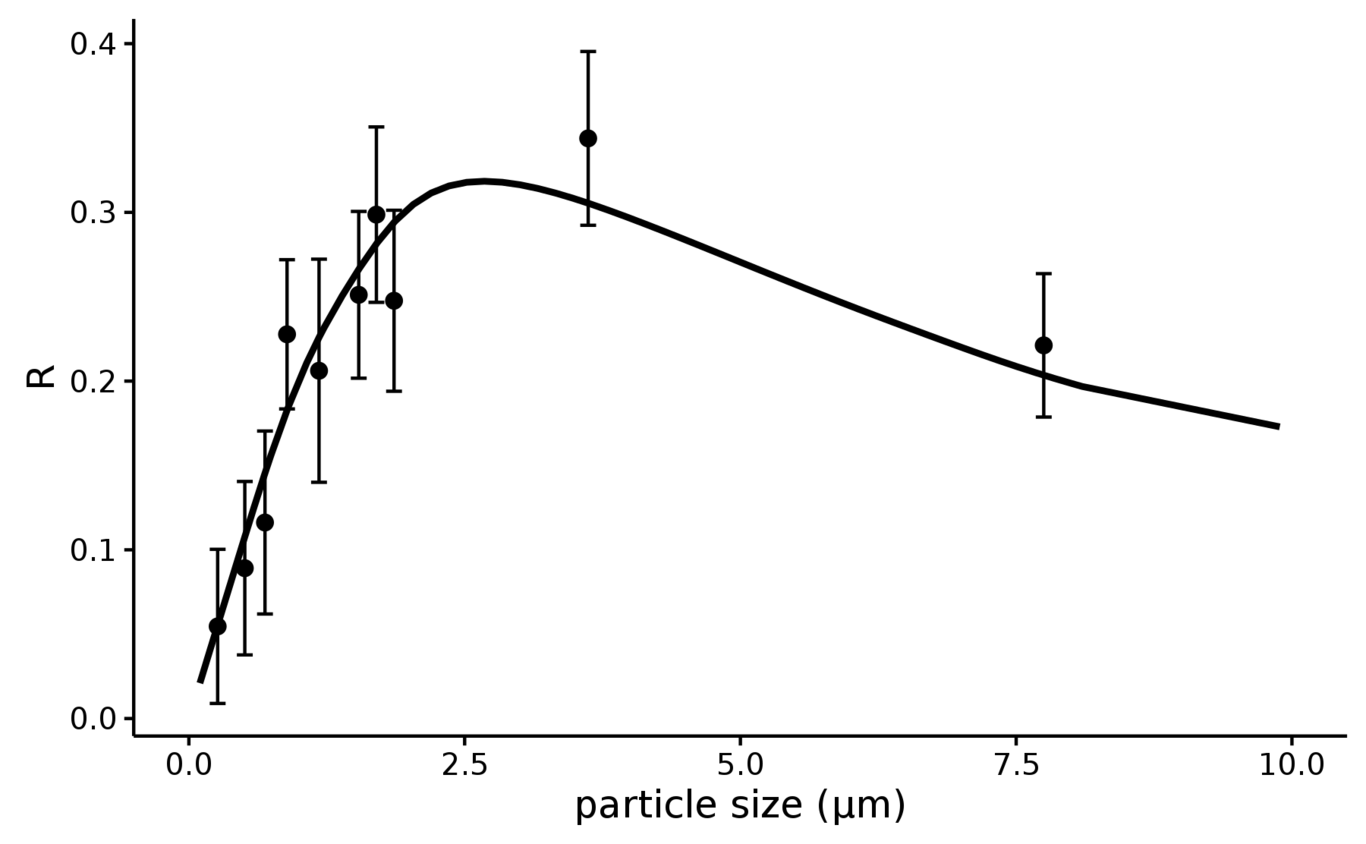
\includegraphics[width=0.70\columnwidth]{gfx/lung-paper-figures/summary/summary}
\caption[Dark-field signals for silicon microspheres.]{Silicon dioxide monodisperse microspheres in a 20\% solution of
    glycerol as a function of sphere diameter. The continuous line is the
    function in eq. {\ref{eqn:lynchpolychromatic}}.
    {\label{725462}}}
\end{center}
\end{figure}

A more general approach links this dark-field extinction coefficient
$\mu_d$ with far-field scattering experiments.
The intensity of the scattered radiation from particles in a solution as a
function of momentum transfer $q$ can be written as~\parencite{PEDERSEN1997171,Gkoumas2016}
\begin{equation}
    I(q) = f|\Delta n| V P(q) S(q),
    \label{eq:scattering.intensity}
\end{equation}
where $V$ is the volume of the particle, $f$ is again the volume fraction
occupied by the particles, $P(q)$ is the form factor of each particle. For a
homogeneous sphere of radius $r$ this function is~\parencite{PEDERSEN1997171}
\begin{equation}
    P(q) = \left[\frac{3(\sin(qr) - qr\cos(qr))}{qr^3}\right]^2.
    \label{eq:sphere.form.factor}
\end{equation}
The function $S(q)$ determines the intensity of interference between
particles. For diluted systems with $f \leq \SI{15}{\percent}$ this can
be neglected, as $S(q) \sim 1$. However, for higher concentrations this term
becomes more relevant, and will reduce the scattering intensity.

Once this scattering intensity function is calculated, the extinction
coefficient can be calculated by taking the Fourier transform of $I$ with respect
to $q$, and by using the classical electron radius $r_e$:
\begin{equation}
\mu_B = (2 \pi r_e)^2 [\Fq I(0) - \Fq I(d)].
    \label{eq:autocorrelation}
\end{equation}

This formula, that we can call the \emph{usaxs method} for the
calculation of the dark-field extinction coefficient, is implemented in a publicly available Python
package~\parencite{scattering-repository}
is used in all the following calculations, where we used the approximation
$S(q) = 1$.

The equivalence between the two calculations can be checked explicitly, for
instance for a system with $p_2 = \SI{2}{\micro\meter}$, $L =
\SI{12}{\centi\meter}$, a solution of silicon dioxide spheres in glycerol
with $f = 0.4$ results in estimates of the dark-field extinction coefficient
according to equations~\eqref{eqn:lynch} and~\eqref{eq:autocorrelation},
which align along the same curve (figure~\ref{fig:equivalence-lynch-saxs}).

\begin{figure}[ht]
    \centering
    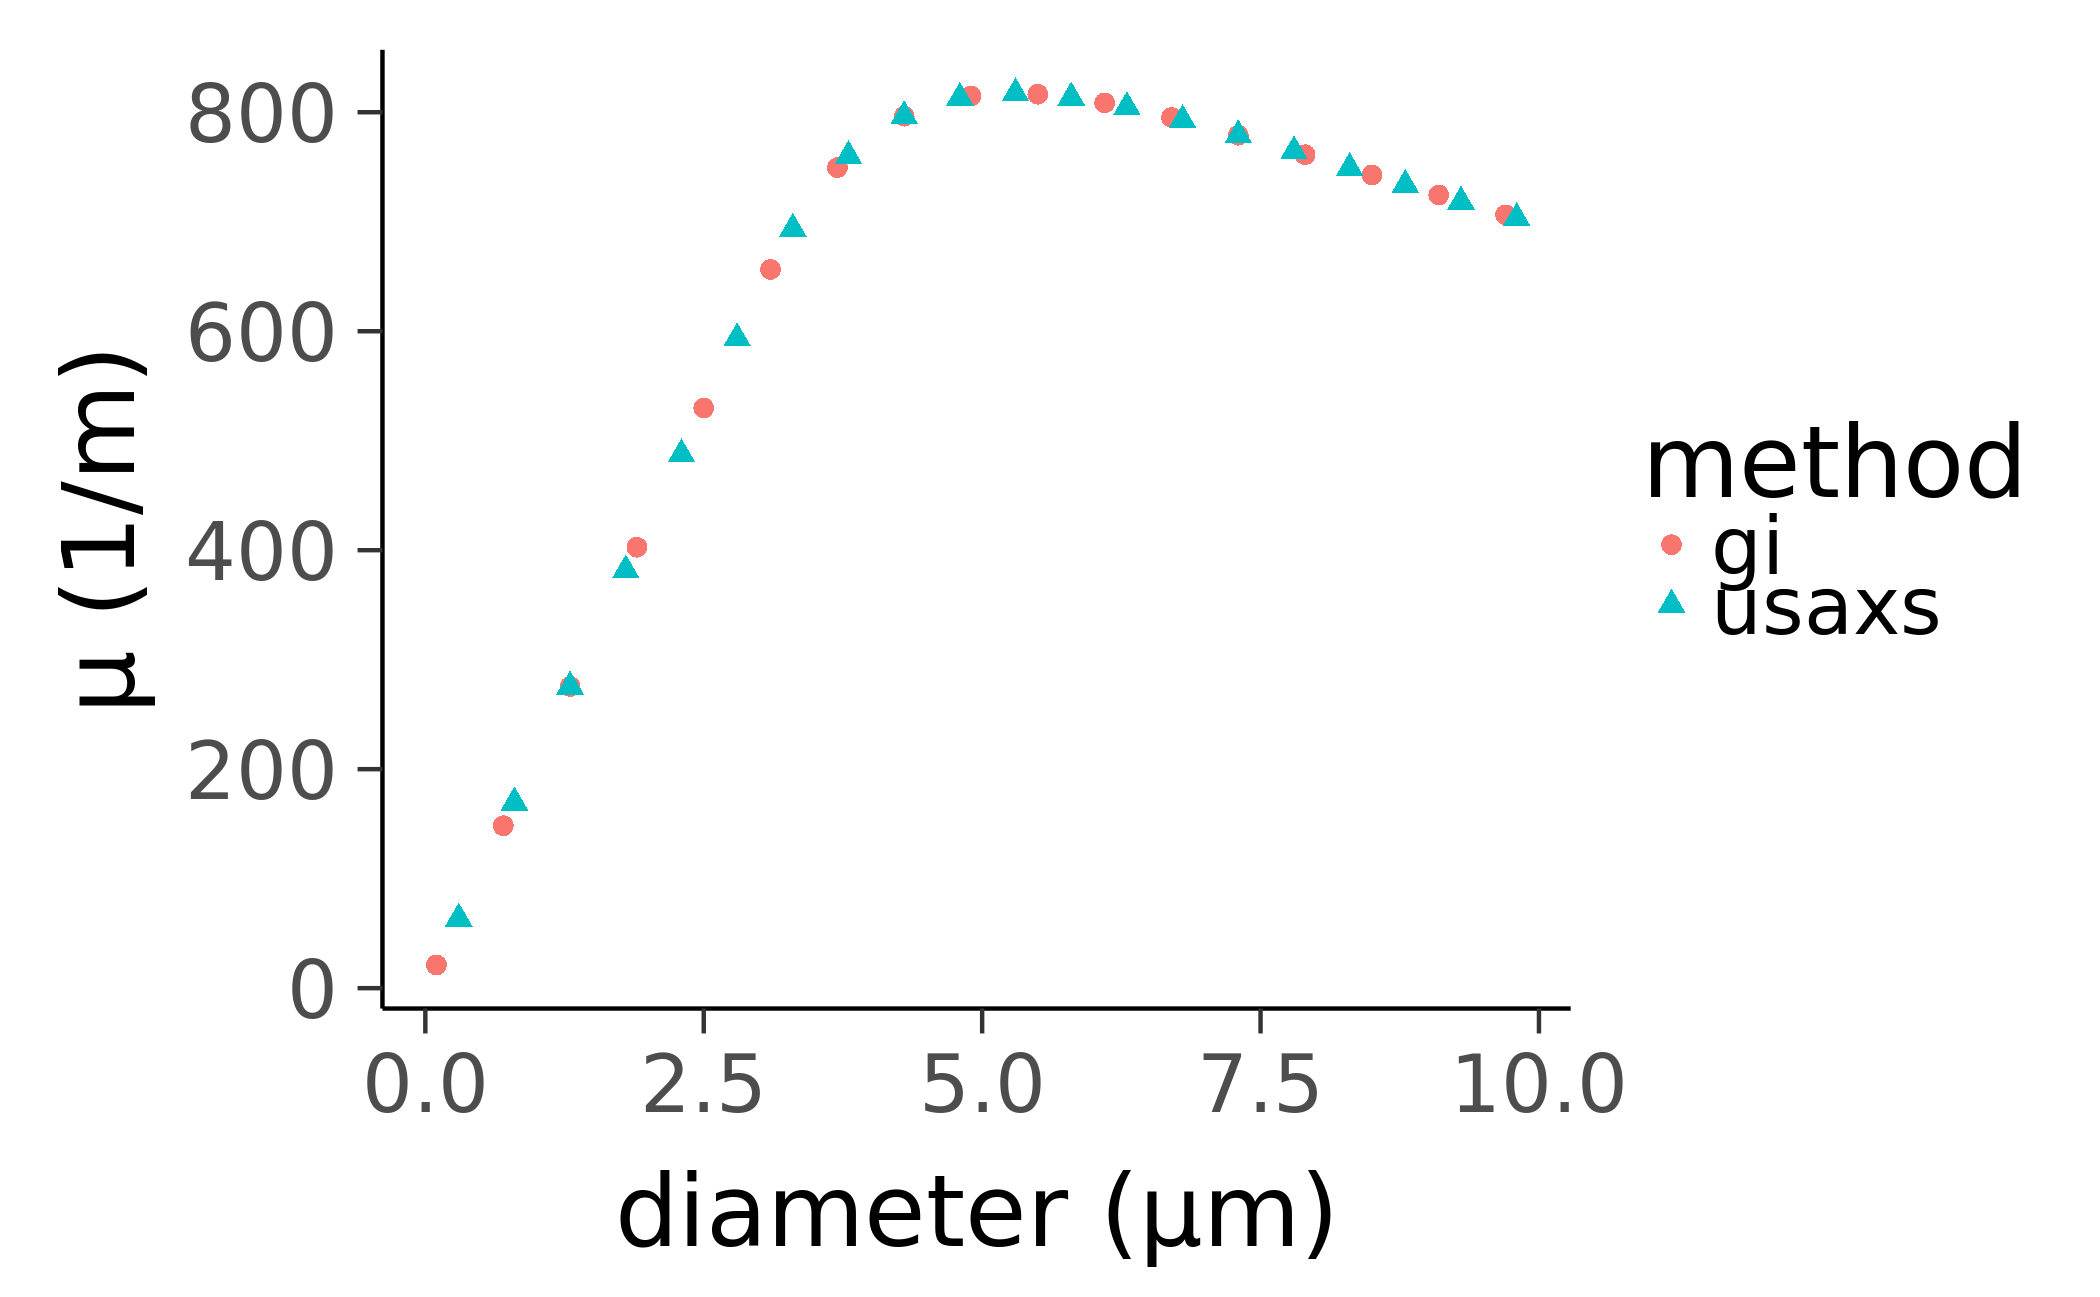
\includegraphics[width=\columnwidth]{gfx/lynch-vs-saxs/plot.png}
    \caption[Equivalence of grating interferometry and small-angle
        scattering approaches for the calculation of dark-field extinction
    coefficients.]{Comparison of equations~\eqref{eqn:lynch}, or \emph{gi} method,
    and~\eqref{eq:autocorrelation}, or \emph{usaxs} method for the
estimation of the scattering intensity, as seen through the dark-field
extinction coefficients. The two methods are equivalent.}
    \label{fig:equivalence-lynch-saxs}
\end{figure}

A model of the sample is required to calculate the spectral weights
$s(\energy)$ in order to avoid beam hardening artefacts. The source spectrum is
simulated with the SpekCalc~\parencite{spekcalc} software, then attenuated
according to NIST absorption tables~\parencite{Hubbell_1995} for the sample in the beam path and the
efficiency of the detector.

In this work, we propose to model the lung sample as a solution of
polydisperse spherical air bubbles embedded in tissue. The distribution of
the sphere diameters is extracted from the microtomographic data
(figure~\ref{fig:sizepdf}),
\begin{figure}[htb]
    \centering
    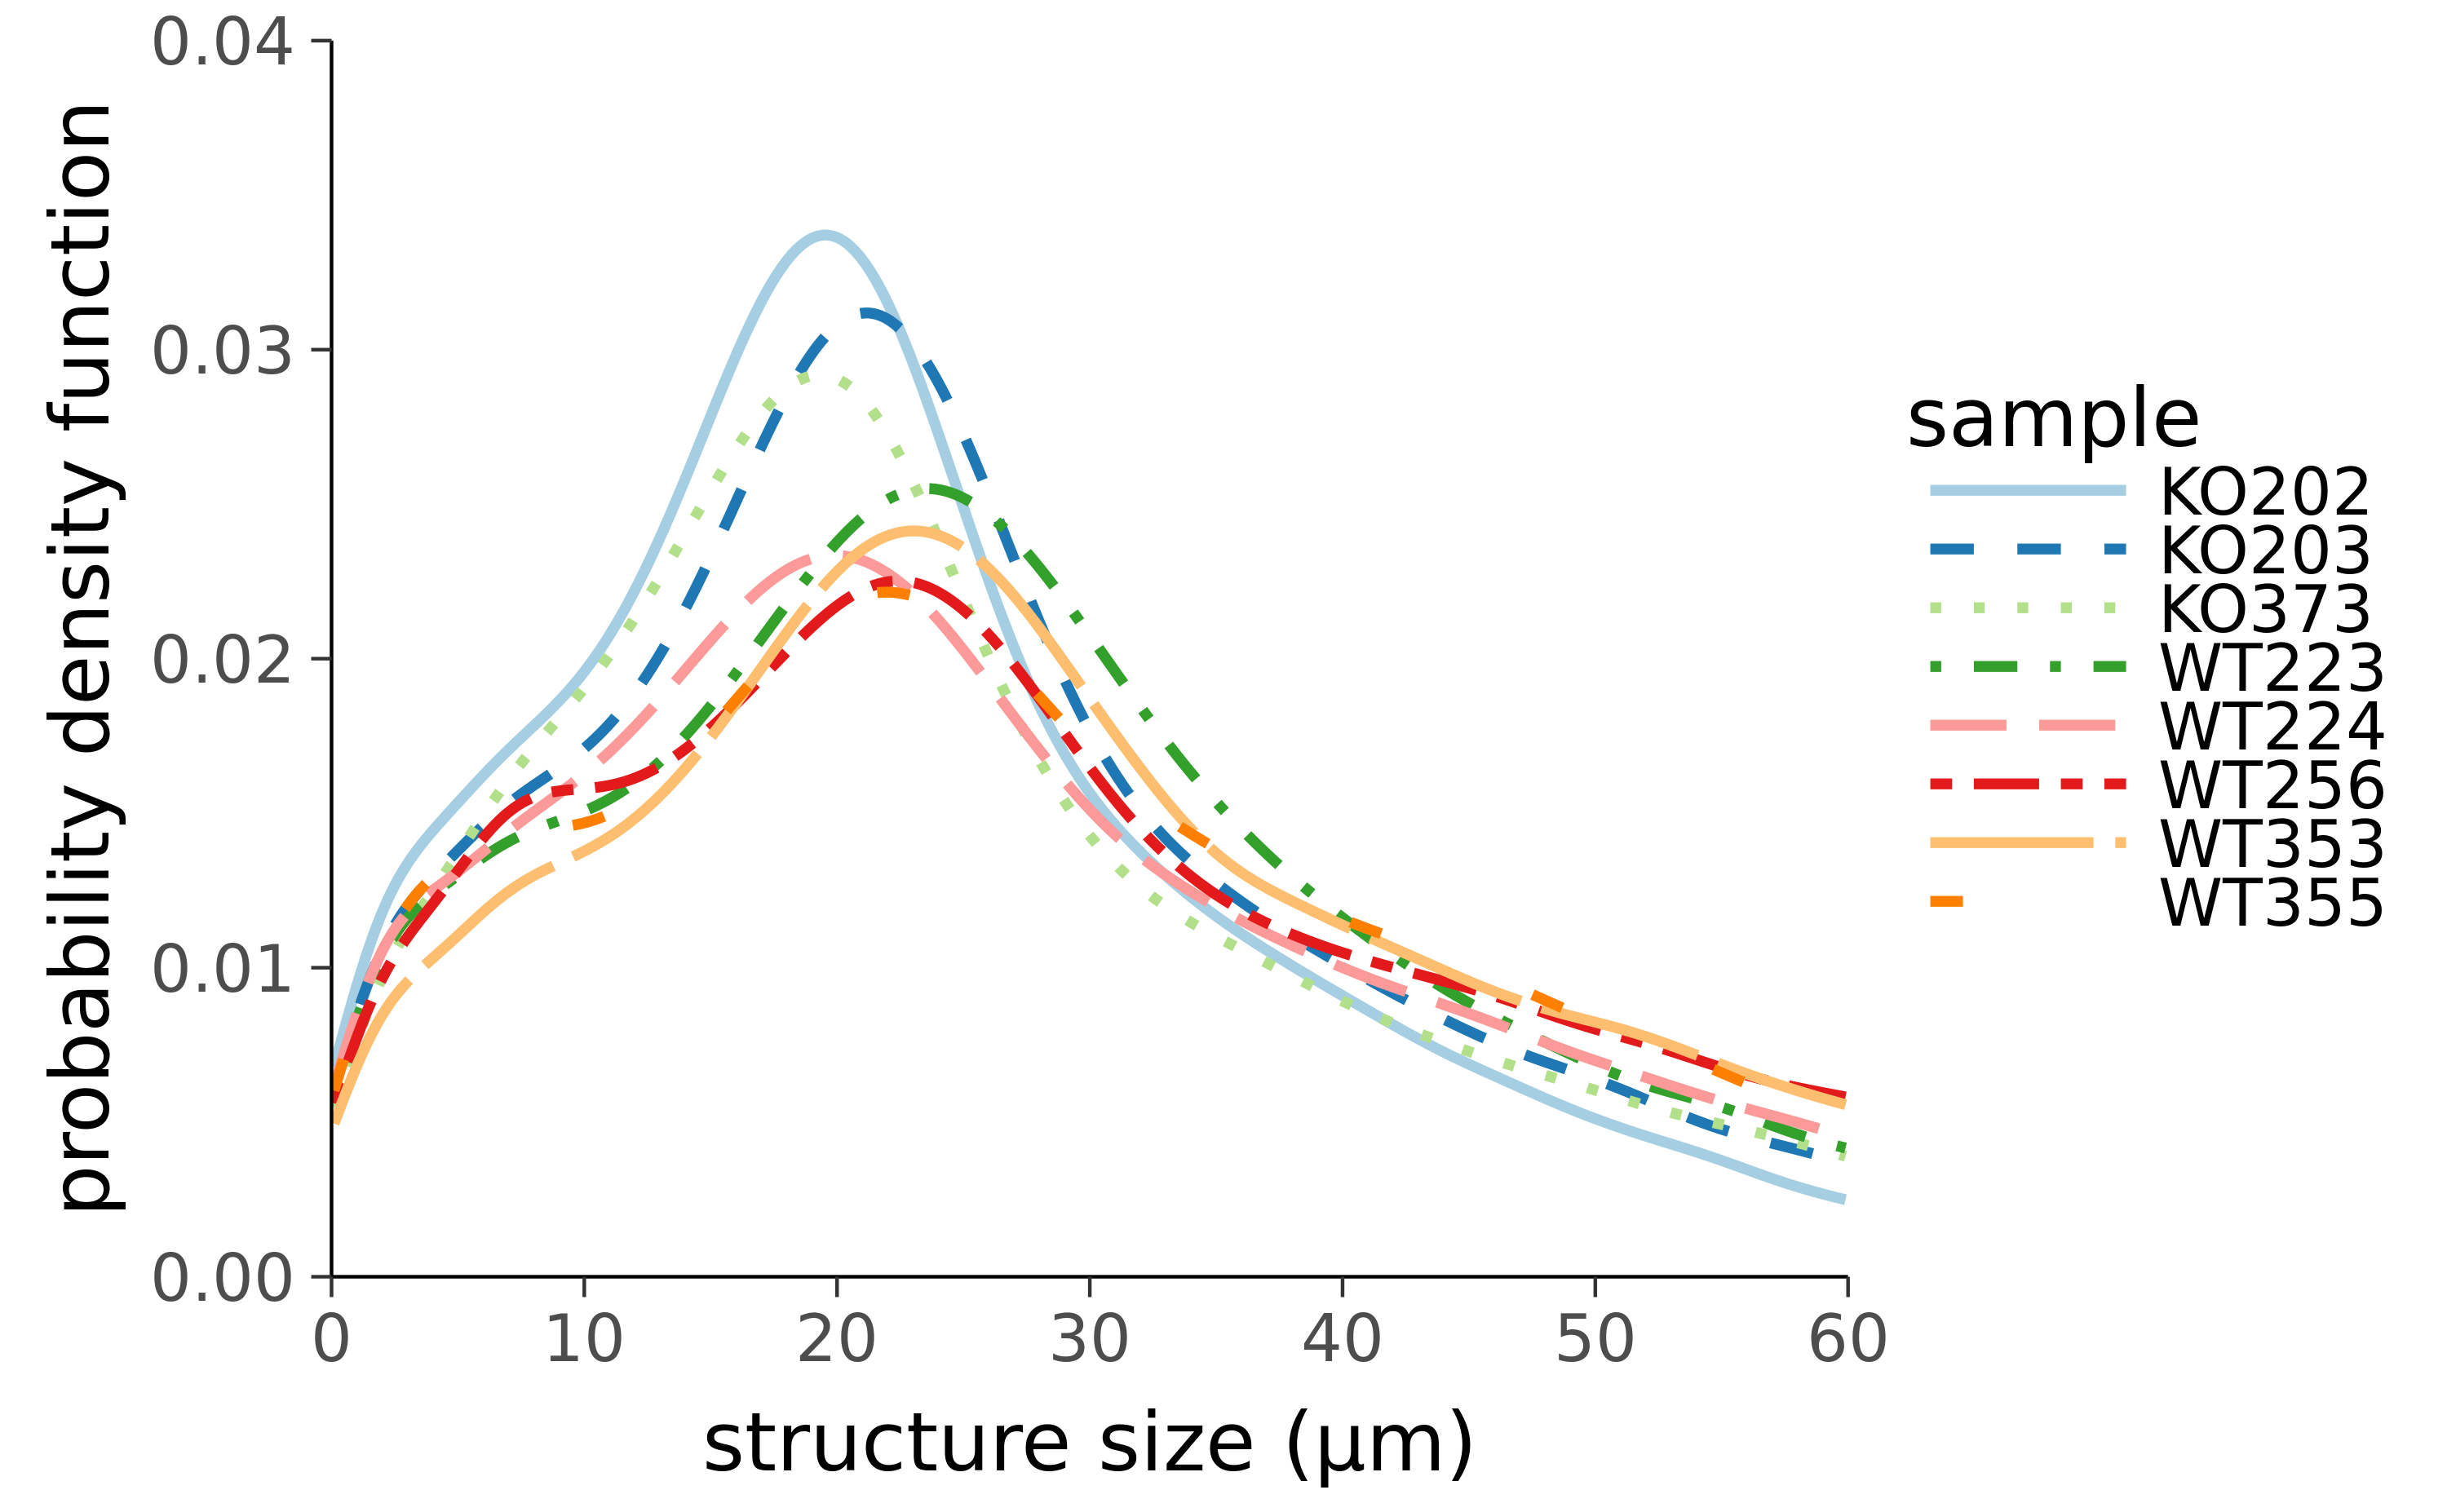
\includegraphics[width=\textwidth]{gfx/lung-paper-figures/size_pdf.png}
    \caption{Distribution of the diameters of the alveoli as determined from
    synchrotron tomography data for all samples.}
    \label{fig:sizepdf}
\end{figure}
together
with the fraction of the volume occupied by the tissue. The density of the
tissue is also estimated from tomographic projections: the composition is
taken from the ICRU-44 lung tissue tables~\parencite{White_1989}, while the density is increased to
1.6 g/cm$^3$ as to match the absorption values recorded on the tomographic
projections. This results from the drying procedure for the fixation of
the samples, leaving a denser material than in \emph{in vivo} conditions.

The coefficient $\mu_B$ can then be expressed as a double summation over the spectrum
$s(\energy)$ and over the distribution of sphere diameters $\rho(d)$:
\begin{equation}
    \mu_{B,\text{total}} = \sum_{d}\sum_{\energy} \mu_B(d, \energy; n, f)\rho(d)s(\energy)
    \label{eqn:totalsum}.
\end{equation}


\section{Results and discussion}\label{sec:results}
The section of the radiographic image of each lung sample is manually
matched to the local tomography, as identified during the alignment of the
tomographic scan. The average and standard deviation of the $R$ values are
calculated and plotted in fig.~\ref{206272} (black dots and errorbars). The expected
values according to eq.~\ref{eqn:totalsum} are calculated with the inputs from the
microtomographic datasets, as described in section~\ref{sec:tomoprocessing}, and are plotted on
fig.~\ref{206272} with red dots for each sample.
\begin{figure}[h!]
\begin{center}
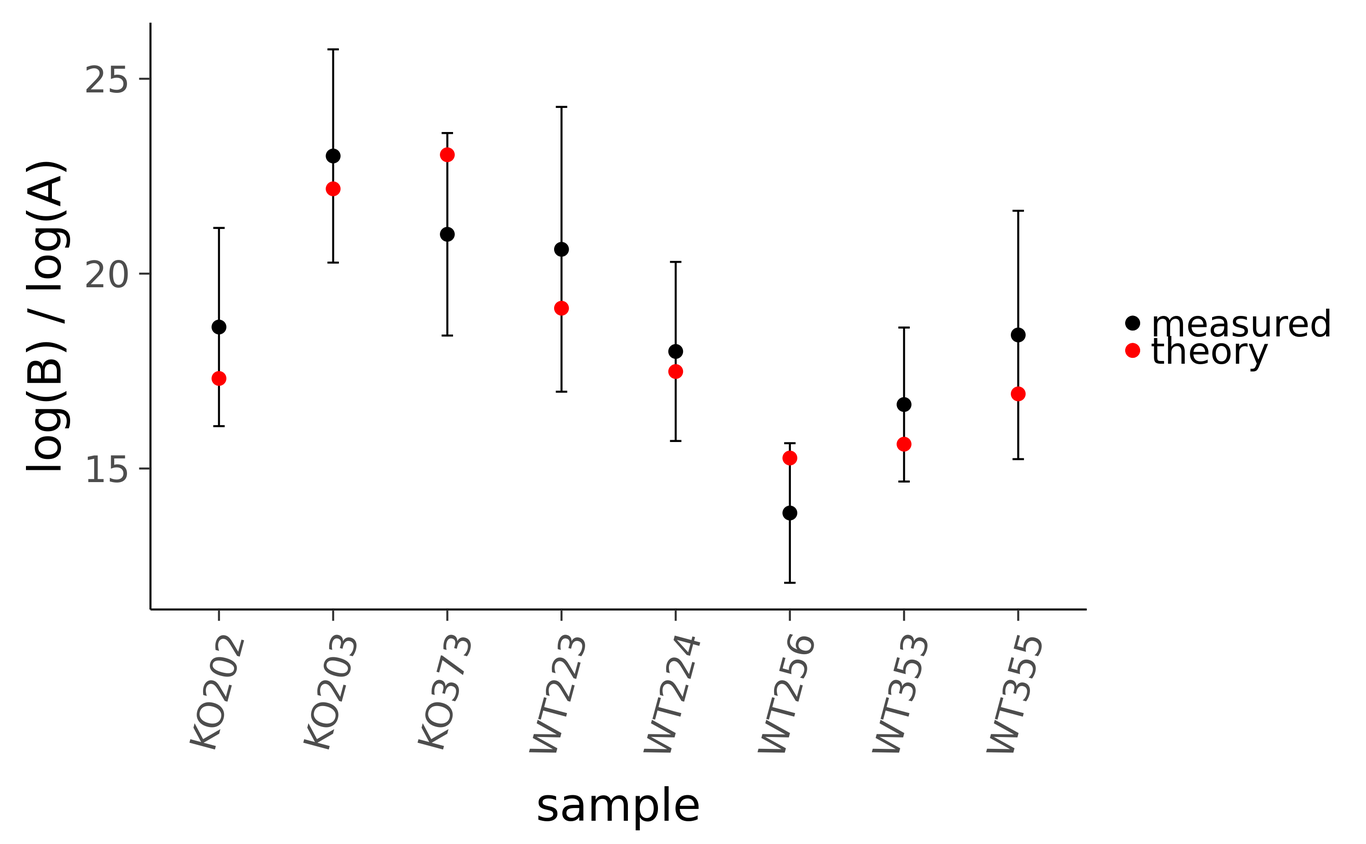
\includegraphics[width=\textwidth]{gfx/lung-paper-figures/samples/samples}
\caption[Comparison of the theoretical estimate and experimental values of
the dark-field signal.]{{\(R\) value for each lung in the laboratory setup
radiography (measured, black dots with errorbars) compared to the
expected value modelled from microtomographic inputs (theory).
{\label{206272}}%
}}
\end{center}
\end{figure}


The measured data agreed with the
theory for all samples, and the $\chi^2$ statistic can be calculated

\begin{equation}
    \chi^2 = \sum_{i=1}^8 \dfrac{(R_{\text{obs}} -
    R_{\text{th}})^2}{\mathop{\mathrm{Var}}(R_{\text{obs}})} = 2.31.
    \label{eqn:chisq}
\end{equation}

With 7 degrees of freedom, this results in a right-tail probability of 0.94 that the 
observations are consistent with the model, thus validating the quantitative estimation of
dark-field values for a lung model as a collection of incoherently
superimposed microscopic spheres.

Possible sources of inaccuracy of our model include a significantly
different distribution of shapes in the lung parenchyma, or additional
effects of beam hardening which are known to influence the dark-field
signal. In order to consider the effects of possible shape asymmetries, a
single mouse lung sample was scanned at the X02DA TOMCAT beamline with the
setup described in~\cite{PhysRevLett.116.093902}. This
technique is similar to Talbot interferometry, but it is able to detect
scattering from unresolved microscopic structures under different angles in
a single shot by
creating an array of circular interference patterns (also see
chapter~\ref{ch:omnidirectional}). The intensity of the
dark-field signals for different angles can then be recovered for each
pixel, and an asymmetry value defined as the amplitude of this periodic
signal divided by the average can be calculated for each pixel. This allows
us to exclude the possibility that there are significant inhomogeneities in
the dark-field response of the lung structures under different angles, which
would directly invalidate the model of a superposition of spheres. This
amounts to quantifying the departure from a spherical model towards
ellipsoids. In our sample this asymmetry is an average of $0.11 \pm 0.04$,
indicating a departure from the spherical model of less
than \SI{15}{\percent}.

Another effect commonly reported in dark-field analyses on wide, polychromatic
sources is the influence of beam hardening on the recorded dark-field
values. In our case, given the high voltage of the source and the small
thickness of the samples (less than \SI{4}{\milli\meter}), the absorption
ranges from \SI{4}{\percent} to \SI{6}{\percent}. The correction to
dark-field values provided by \cite{Yashiro:15} is therefore
not applied, as it is reported to be relevant for samples absorbing at least
50\% of the incoming light. The beam hardening effect is considered insofar
it affects the spectral weights of eq.~\ref{eqn:totalsum}, which are calculated
after the sample. 

\section{Water diffusion in cement: an application to material science}
One of the applications of grating interferometry to material science is the
study of diffusion of gas or water through porous materials, such as motor
catalytic filters~\parencite{doi:10.1021/cs3004006} or diffusion of water through cement~\parencite{20.500.11850/268}.

We reproduced this result with the following experiment, where a cement
cylinder is sealed on the sides and put in contact with a water layer on the
bottom. The water slowly infiltrates the porous structures with time, and
the height of the water column $h$ can be modeled with a simple
proportionality to the square root of the time $t$ elapsed since the beginning
of the experiment
\begin{equation}
    h = C\sqrt{t}.
    \label{eq:sorptivity}
\end{equation}

Repeated radiographies are taken with \num{20} phase steps and an exposure
time of \SI{0.2}{\second} per step, as the evolution of the sample is
recorded for a period of time of two hours. Figure~\ref{fig:wet-cement}
shows a comparison in the transmission and reconstructed ratio $R$
(equation~\ref{eqn:definitions}) for the first scan and after one hour.

\begin{figure}[htb]
    \centering
    \begin{subfigure}[b]{.49\textwidth}
    \centering
    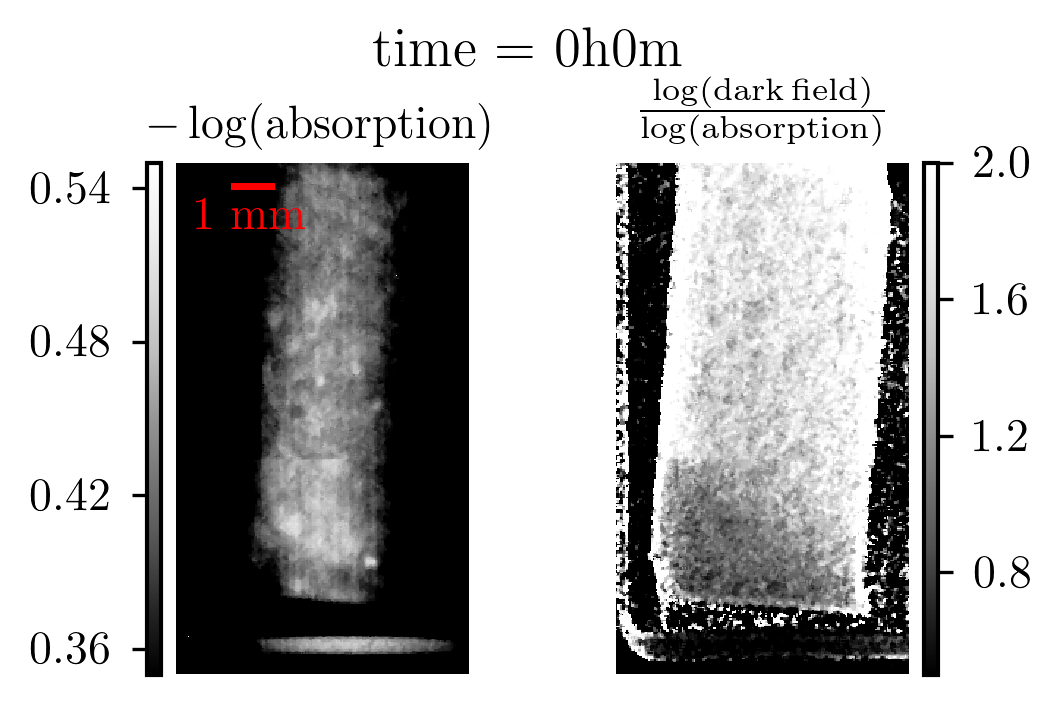
\includegraphics[width=\textwidth]{gfx/wet-cement/0.png}
    \caption{}
    \label{fig:wet-cement-0}
    \end{subfigure}
    \hfill
    \begin{subfigure}[b]{.49\textwidth}
    \centering
    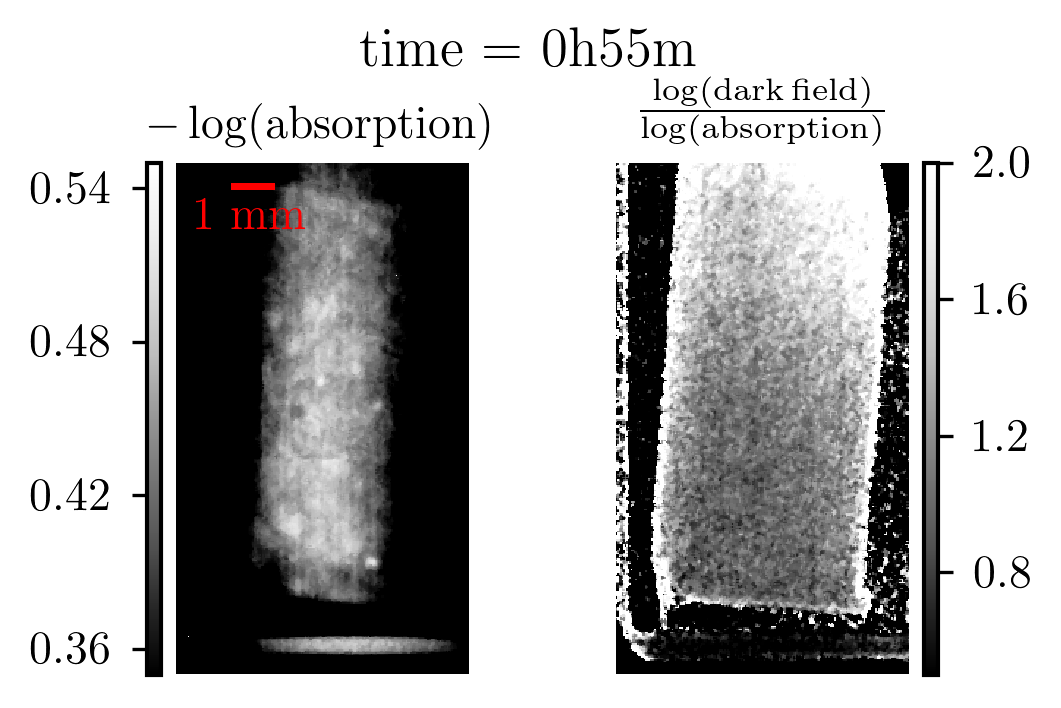
\includegraphics[width=\textwidth]{gfx/wet-cement/200.png}
    \caption{}
    \label{fig:wet-cement-200}
    \end{subfigure}
    \caption[Water uptake in cement.]{Transmission and ratio $R$ for the
    water uptake in a cement cylinder as a function of time: first scan at
$t=0$ (left) and after one hour (right). The fraction of the cylinder
infiltrated by water can be determined with a larger contrast-to-noise ratio
on the $R$ image than in the conventional transmission image (also see
figure~\ref{fig:wet-cement-cnr}).}
\label{fig:wet-cement}
\end{figure}

Figure~\ref{fig:wet-cement-cnr} shows the contrast-to-noise ratio between a
region of the sample that is still dry against a region containing water. It
is clear that the additional contrast provided by dark-field imaging is
beneficial to this kind of analyses.
\begin{figure}[htb]
    \centering
    \begin{subfigure}[b]{.49\textwidth}
    \centering
    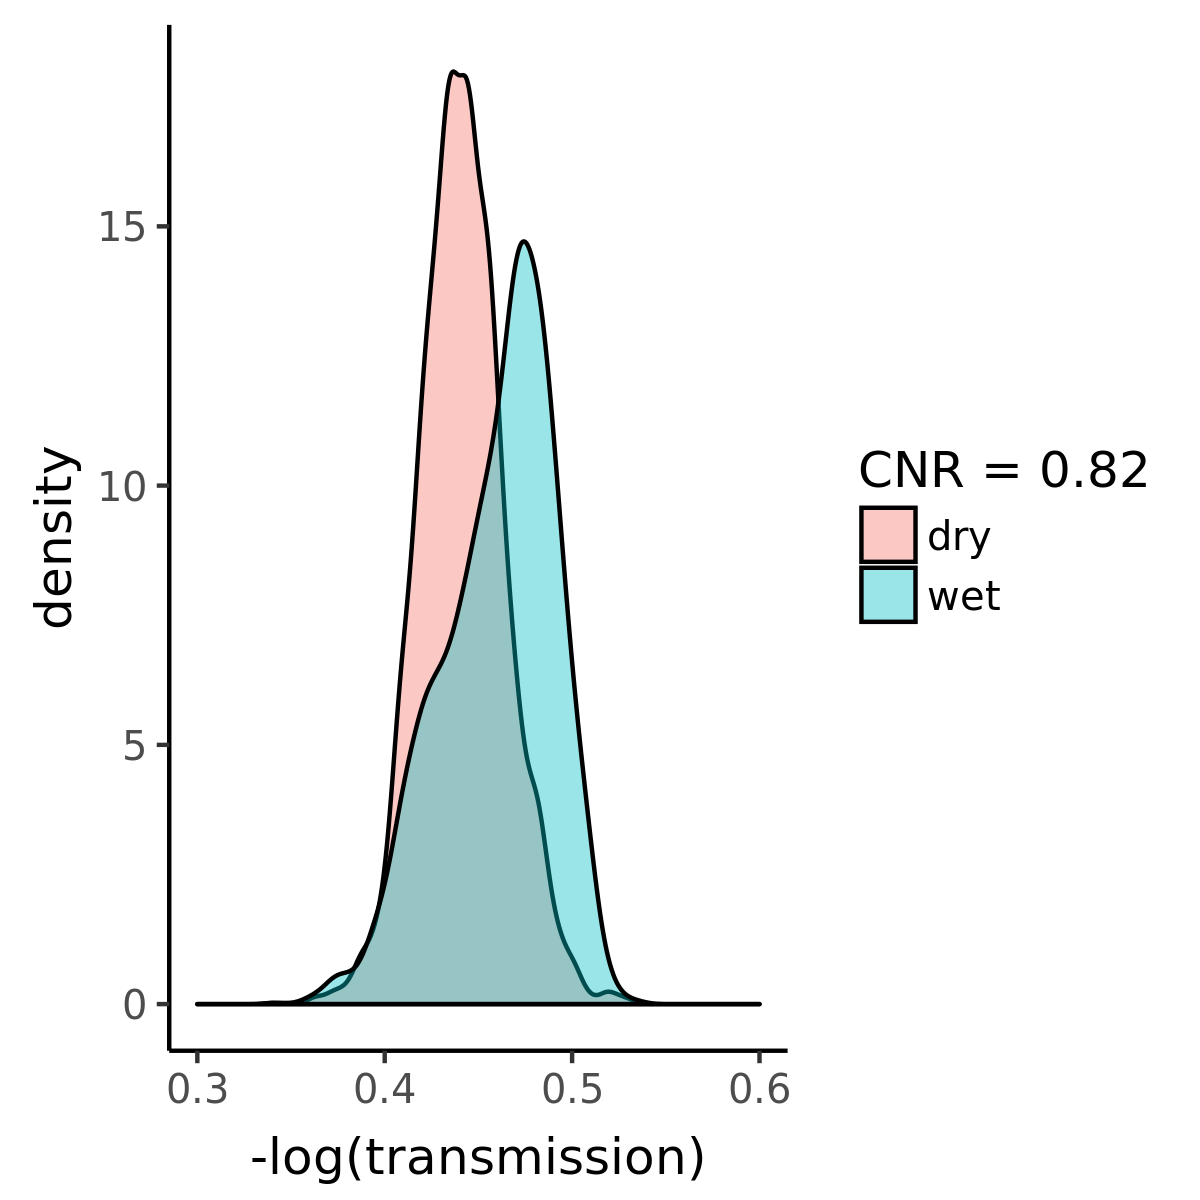
\includegraphics[width=\textwidth]{gfx/wet-cement/cnr_absorption.png}
    \caption{}
    \label{fig:wet-cement-cnr-absorption}
    \end{subfigure}
    \hfill
    \begin{subfigure}[b]{.49\textwidth}
    \centering
    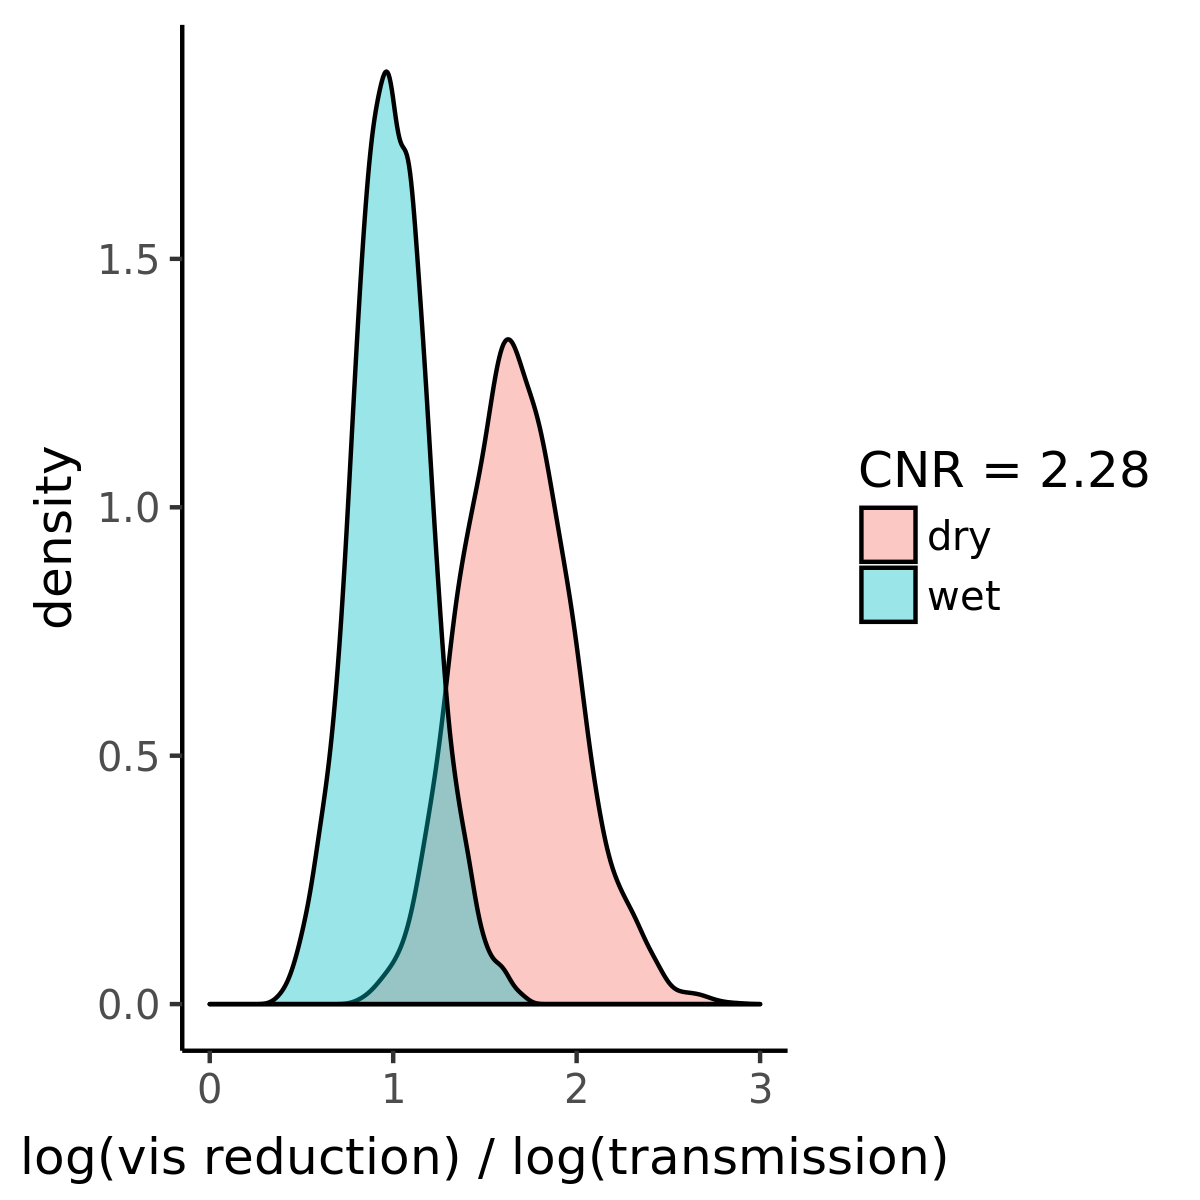
\includegraphics[width=\textwidth]{gfx/wet-cement/cnr_ratio.png}
    \caption{}
    \label{fig:wet-cement-cnr-ratio}
    \end{subfigure}
    \caption[CNR for water in cement.]{Comparison of the contrast-to-noise
    ratio between a manually selected wet and dry region in transmission and
ratio $R$.}
\label{fig:wet-cement-cnr}
\end{figure}

Finally, these data can be combined together to confirm the relationship in
equation~\eqref{eq:sorptivity}: the histogram of the ratio images are
calculated and thresholded, the pixels below the threshold are
counted as wet pixels, the pixels above the threshold count as dry. The
resulting fit is shown in figure~\ref{fig:position}, confirming the
square root proportionality between the height of the water column and time.

\begin{figure}[htb]
    \centering
    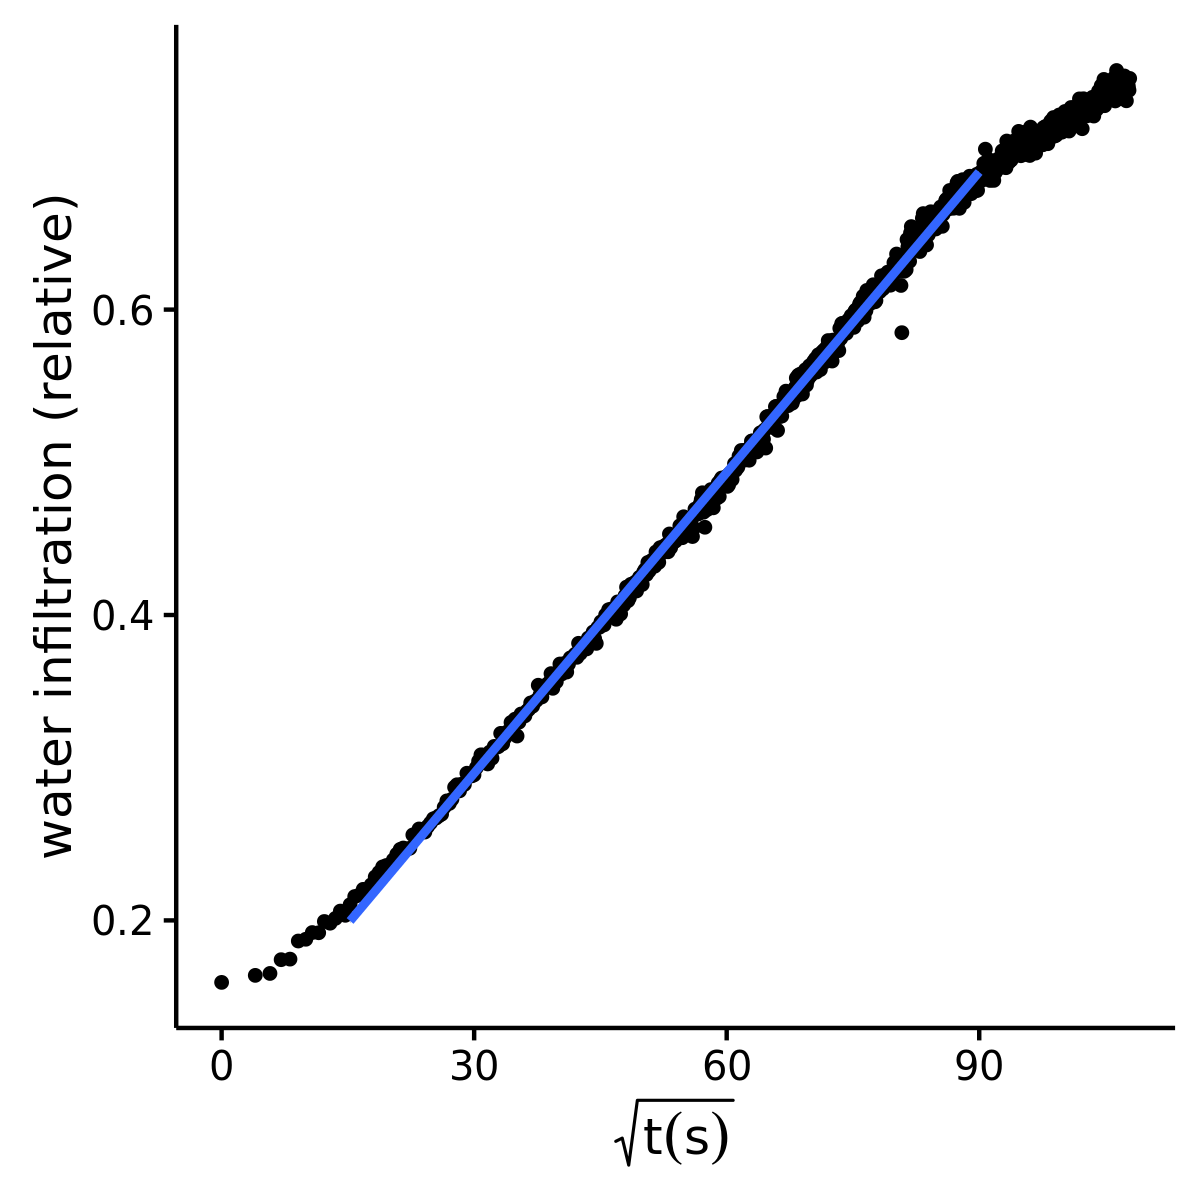
\includegraphics[width=\textwidth]{gfx/wet-cement/position.png}
    \caption[Water diffusion in cement.]{Height of the water column in a cement cylinder as a function
        of time, measured on $R$ images from the \SI{45}{\kilo\eV} grating
    interferometer. The blue line is a linear fit according to
    equation~\eqref{eq:sorptivity}, establishing the proportionality between
the square root of the elapsed time in the experiment and the height of the
water column infiltrating a porous material.}
    \label{fig:position}
\end{figure}

\section{Conclusion}
In this chapter we were able to show quantitative measurements using the
dark-field signal from laboratory sources. In particular, a mouse lung is
modelled as a collection of spheres with a distribution of diameters determined
by microscopic tomography on the X02DA TOMCAT beamline. This distribution is
then weighted by the expected dark-field response of the instrument; it can
be proven that this matches the dark-field values as measured on a
polychromatic laboratory source radiography collected with an exposure time
of \SI{31}{\second}.

While this setup has a short autocorrelation length of only few micrometers
(figure~\ref{725462}), it would be possible to design a setup that is more
sensitive to the structure sizes found in human lungs, where the alveoli are
larger than
\SI{100}{\micro\meter}~\parencite{doi:10.1164/rccm.200308-1107OC}. Without excessively stretching the
requirements for the fabrication of the optical elements, we can describe a
possible choice of parameters for a Talbot-Lau interferometer for lung
screening. The design energy can be chosen as \SI{60}{\kilo\eV}, close to
the mean energy for a \SI{100}{\kilo\voltpeak} setting on a chest
radiography. An intergrating length of \SI{1}{\meter} is required to provide
enough room for the patient to comfortably fit the machine,
and a period of \SI{1.2}{\micro\meter} could be achievable without
excessively stretching the requirements on the fabrication of the optical
elements. This results in an autocorrelation length around
\SI{25}{\micro\meter}, which is large enough to provide contrast according
to the mechanism shown in figure~\ref{725462}, thus providing better contrast than the
current setup, which was not originally designed for an application to human
diagnosis.
This would have the potential to provide a replicable and quantitative
structural assessment of the lung parenchyma down to the smallest components
with a fast scan, with potential benefits to the early diagnosis of
emphysema and lung cancer, which is critical for an effective treatment of
this class of diseases.
